\chapter{\label{ch:2-elastic}\chelastic} 

\minitoc

\section{Introduction}

Biological membranes are abundant and are crucial to cellular and sub-cellular organisation. Membranes allow for the spatial and temporal management of reactions and the separation of substances and environments \cite{simunovic_when_2015}. In addition to the familiar cellular membrane, eukaryotic cells also contain internal membranes that form the boundaries of organelles such as mitochondria, chloroplasts and lysosomes \cite{zimmerberg_how_2006}. Biological membranes are sheet-like lipid bilayers that are two molecules thick (4-10nm) \cite{berg_biochemistry_2002}. These are dynamic, fluid structures in which proteins float in a sea of lipids diffusing in the plane of the membrane and different composition of these proteins and lipids can generate asymmetry across the membrane. In addition to compartmentalisation, biological membranes serve several additional functions necessary for life, such as energy storage and information transduction, and many of these are dictated by the proteins associated with them.

Membranes are also a central focus in the development of novel biotechnology and biologically inspired materials. For example, surrounding substances with lipid bilayer membranes can create small compartments called liposomes that can aid in drug delivery \cite{lasic_applications_1995}. More recently, the development of DNA origami \cite{rothemund_folding_2006} has allowed for the engineering of sophisticated biomimetic systems of membranes that can control adsorption. These membranes are also candidates for controllable barriers, with engineered DNA nanopores displaying gating properties similar to natural ion channels and switch between open and closed states depending on the transmembrane voltage \cite{seifert_bilayer-spanning_2015}. Conventional engineered systems often rely on materials with specific properties at the atomic/molecular scale, but lack the hierarchical structure of interacting building blocks to enable macroscopic dynamic behaviour which is seen in biology \cite{studart_biologically_2015}. Tuneable and functional modules with active membranes may provide a scheme to develop these types of systems \cite{czogalla_dna_2016}. Additional to controlling the permeability of membranes, origami structures mimicking membrane-sculpting proteins have also been reported \cite{czogalla_amphipathic_2015} and present the possibility of controlling the shape of membrane bound compartments. Understanding more about the forces that govern the behaviour of membranes will therefore not only aid understanding of biophysical processes, but will also help to direct future bioengineering.

The shape of membranes is crucial to development and function. The endoplasmic reticulum (ER) and the Golgi apparatus have very complex boundaries defined by the curvature of the internal membrane, however they have distinctly different shapes. Both structures have very large surface area for their volume, however the ER is more tubular compared to the more saccular Golgi apparatus \cite{zimmerberg_how_2006}. This difference in structure may be related to the different functions of these organelles or as a consequence of the material within the organelle. Regardless, in order to understand the physical origin of these shapes, it is crucial to understand the interplay of the membrane with other biomolecules and structures and in particular the proteins embedded or tethered to the membrane. Membrane-bound proteins have been shown to be directly connected to membrane curvature and also to function, for example endocytosis being controlled by curvature inducing proteins that curve the membranes to form vesicles and allow the cell to take in external substances by engulfing the material \cite{boucrot_endophilin_2015}.

Different mechanisms can control the changes in membrane shape, for example transporter proteins that can generate forces by moving material across the membrane, or the cytoskeletal structure can pull on the membrane \cite{ghosh_pattern_2021}. These forces act to change the natural shape of the elastic membrane which  is stiff and resists shape changes away from a rest configuration. Deformations in the membrane shape can also be caused by a variety of curvature inducing inclusions, such as proteins that can bind to the membrane and insert structures that wedge the membrane and cause a bend \cite{simunovic_when_2015, argudo_continuum_2016}. Two or more of these inclusions can then interact elastically, as the membrane responds to a curvature that is locally imposed by each inclusions. Since these proteins are also able to move within the fluid membrane, they will respond to forces pulling them together or pushing them apart to minimise the energy of the global deformation.

The Bin/amphiphysin/Rvs (BAR) domain proteins are a common family of curvature inducing membrane proteins that have a curved domain and induce curvature on the membrane by binding to it. BAR proteins are involved in many cellular processes and they can both sense the curvature of the membrane and also influence the membrane shape. Different BAR domains have different shapes and this can cause different deformations in the membrane. One common feature across the BAR domains is that they are not rotationally symmetric and so the the proteins impose more complex constraints on the membrane than simple bowl like deformations. This anisotropy is essential to the formation of membrane tubules, as symmetric deformations imposed by bowl-like proteins, such as clathrin, form spherical vesicles instead \cite{simunovic_when_2015}. Thus, it is crucial to understand the elastic interactions between anisotropic proteins to gain insight into how membrane elasticity influences the cellular environment.

Prior work has studied the role of elastic interactions between membrane bound curvature inducing inclusions \cite{argudo_continuum_2016, helfrich_elastic_1973, kim_curvature-mediated_1998, brown_elastic_2008}. Different models assume different membrane tensions, inclusions separations and inclusion shape. One alternative to describing the distribution of individual interacting inclusions is to study the evolution of a density field that describes the distribution of curvature inducing inclusions on the surface of the membrane. Continuum models \cite{agudo-canalejo_pattern_2017} have been developed to study the stability of a uniform distribution of curvature inducing particles on a spherical vesicle. In addition to the elastic energy, the continuum framework is amenable to adding additional effects, such as the correlation of fluctuations, additional inclusion-inclusion interactions and even to couple the resulting deformations to the actomyosin cortex and other important cellular structures/processes \cite{ghosh_pattern_2021}. Growing instabilities in the distribution of curvature inducing inclusions may act to co-localise membrane proteins and to drive large scale shape changes in the cell \cite{garcia-lara_supramolecular_2015}.

However these top-down density field models do not specify any details of the mechanisms behind these interactions. This would be useful to know, to investigate specific regions of parameter space that correspond to the parameters observed in vivo. Understanding the mapping from individual particle properties to the parameters in the density description would present a new way to measure these small scale properties, provide alternative verification of current measurement techniques, or highlight broken symmetries from anisotropic curvature inducing inclusions. At very high densities of inclusions, interactions preventing inclusions from overlapping can drive the formation of a nematic phase \cite{tozzi_theory_2021}. However at lower densities, when the separation between these inclusions is large, the elastic interaction is less intuitive and the role of tension that resists deformations further complicates the interactions. This is the situation we study here, a system of interacting inclusions that are well separated embedded in a membrane with tension. This study is motivated by biological observations, however the results will also hopefully add another mechanism for the control of interactions of synthetic membranes and the formation of structures from individual inclusions.

\begin{figure}[h]
\centering
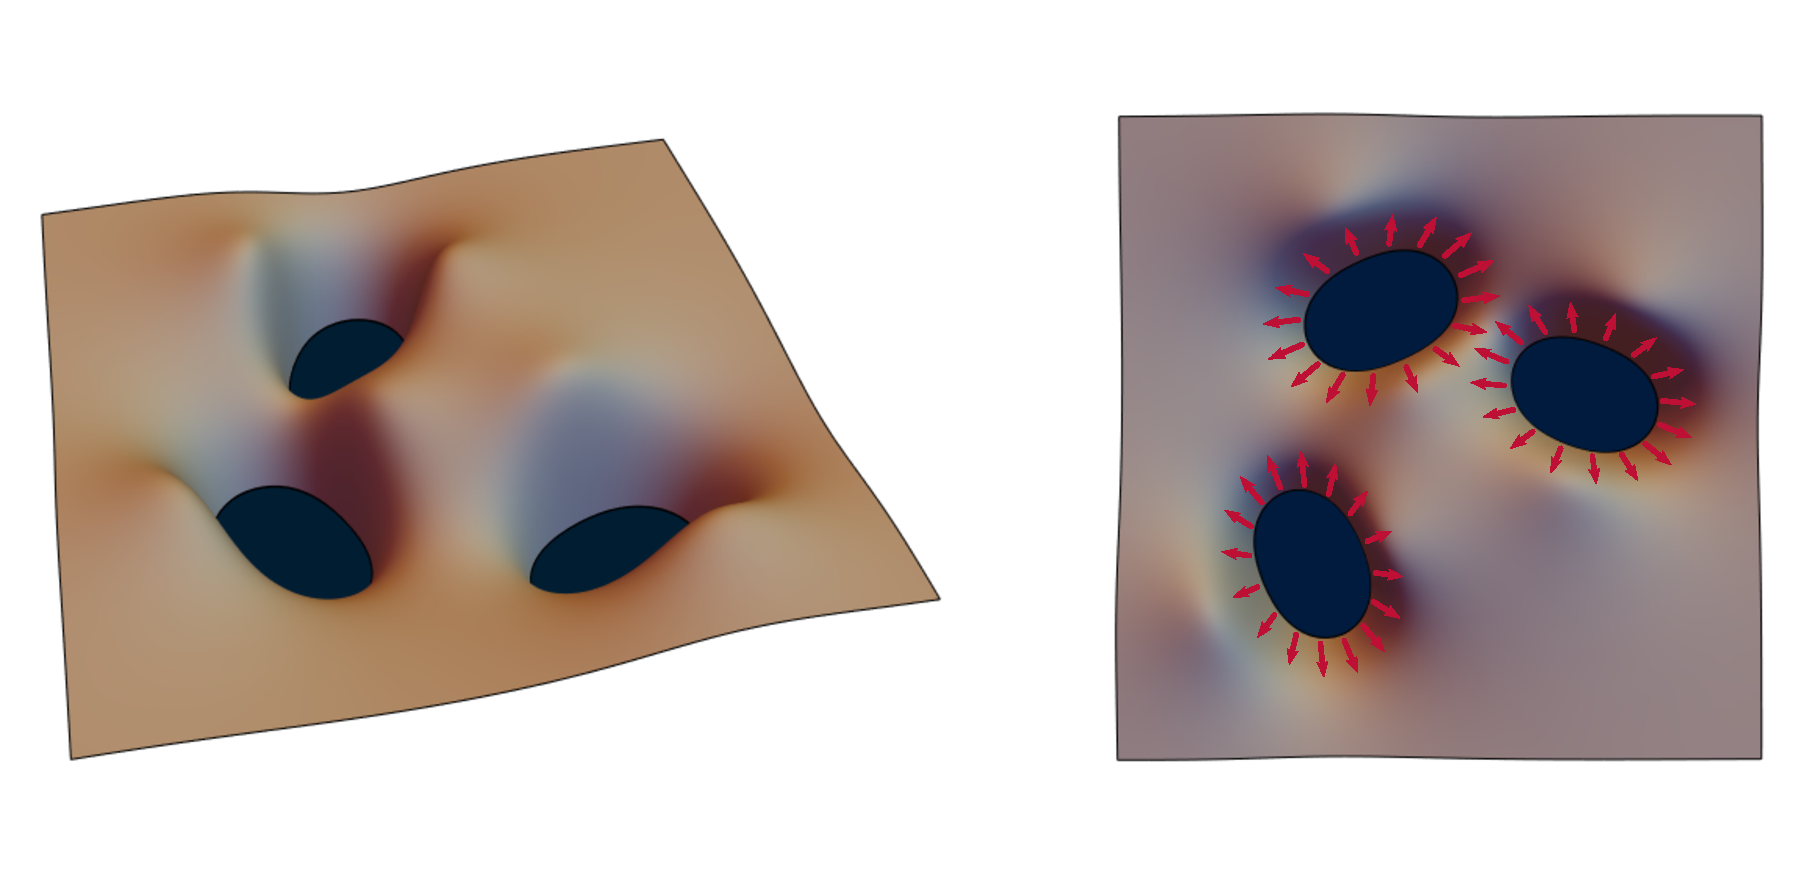
\includegraphics[width=12cm]{figures/3-elastic-figs/threeinc_scheme.pdf}
\caption{Example of three inclusions embedded in an elastic membrane and the resulting membrane shape from two different angles. The inclusions can interact via the elastic mediate membrane forces.}
\label{fig:overview}
\end{figure}

\subsection{Interactions of Anisotropic Inclusions}

Kwiecinski, Goriely and Chapman (KGC)\cite{kwiecinski_interactions_2020} described the interaction between two asymmetric inclusions by considering a circular inclusion that constrains the contact angle with the rest of the membrane, $\tilde{\alpha}$. The inclusions have radius $\epsilon$ and are typically separated by a distance $L$, such that $\epsilon \gg L$. Symmetric inclusions will have a constant contact angle, however in the anisotropic case the contact angle at the edge of the inclusion may vary and this gives the inclusions an orientation. The authors studied the case where the contact angle, $\tilde{\alpha}$, is
\begin{equation}
    \tilde{\alpha}=\tilde{\alpha}^{(0)} + \tilde{\alpha}^{(2)}_i\cos2\phi,
\end{equation}
and $\phi$ is the angular position on the edge of the inclusion (there is no term $\sim\cos\phi$ as this corresponds to tilting the membrane and does not contribute to any interaction energies). Surprisingly, breaking the symmetry of the inclusion results in an equilibrium separation between two interacting inclusions, where the interaction energy is locally minimised. This is a fundamentally different behaviour to the exclusively repulsive interactions seen by symmetric inclusions. Here we study a generalisation of this model to multiple interacting inclusions and study the effects of the broken symmetry and equilibrium inclusion separation.

\begin{figure}[h]
\centering
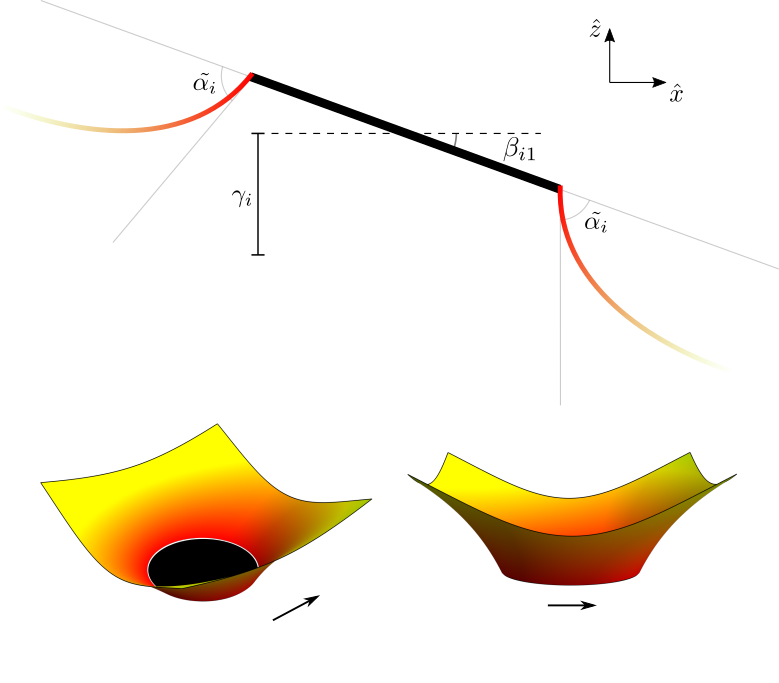
\includegraphics[width=12cm]{figures/3-elastic-figs/conttil.png}
\caption{Contact angle induced by a circular inclusion. The top scheme shows a cross section of the inclusion. The bottom two surface plots show the membrane response locally to an anisotropic inclusion, where the arrow indicates the orientation.}
\end{figure}

\section{Background}

\subsection{Helfrich Hamiltonian}

A common approach to describe the response of an elastic sheet to deformations is to use a Hamiltonian describing the energy of the membrane. The resulting physical system minimises this energy subject to the constraints of the bending \cite{deserno_fluid_nodate}. We can use the Helfrich Hamiltonian to calculate energy of a particular membrane geometry, described by the mean curvature $H$ and Gaussian curvature $K_G$. Additionally, the two monolayers in biological membranes can have different lipid composition and this can cause the rest configuration to no longer be flat and results in the bilayer having some non-zero intrinsic mean curvature, labelled $H_0$. This gives the energy of a membrane $E$ to be
\begin{equation}
    E = \int_{\Omega}\underbrace{\frac{\kappa}{2}(H-H_0)^2 + \overline{\kappa}K_G + T}_{\text{Helfrich Hamiltonian}}\text{d}A
    \label{helfrich}
\end{equation}
where $\kappa$ is the bending stiffness, $\overline{\kappa}$ is the saddle-splay modulus, $T$ is the tension and the integral is taken over the whole membrane, $\Omega$ \cite{kwiecinski_interactions_2020}. In this work, we consider $\Omega$ with fixed topology and with constant surface normal direction at the boundary of any inclusions. As such, the Gauss-Bonnet theorem gives the contribution from the Gaussian curvature, $K_G$, as only contributing a constant and thus not affecting the subsequent physics \cite{deserno_fluid_nodate}, unless there is a change in the membrane topology.

\subsection{Monge Parameterisation}

Cell membranes are much larger than curvature inducing inclusions (often these inclusions are simply proteins). Giant vesicles are used in many experiments on the physics of membranes and are smaller than cells, around \SI{20}{\micro\metre} in size,\cite{ramaswamy_nonequilibrium_2000} many times larger than the \SI{22}{\nano\metre} diameter of the abundant curvature inducing Bin/ amphiphysin/ Rvs (BAR) domain \cite{peter_bar_2004}. At the scale of the protein we therefore expect membranes to appear locally as planes with small regions of curvature induced by inclusions. As the proteins interact and potentially accumulate, or other cellular mechanisms force the membrane to curve this approximation may break down, but the assumption of a flat membrane provides a useful regime to explore the onset of these affects and allows us to use a Monge parameterisation to describe the surface \cite{deserno_fluid_nodate}. The Monge parameterization describes every point on a membrane $\textbf{r}=(x,y)$, as having height $\xi h(\textbf{r})$ above a reference plane (at $h=0$). Taking $\xi \ll 1$ this parameterisation describes surfaces that have small deformations and no overhangs. Additionally, we can nondimensionalize the position and the height by an arbitrary length, $L$. This choice allows us to write the mean curvature of the membrane, $H$, in terms of $h(\textbf{r})$ to give
\begin{equation}
    H = \nabla\cdot\Bigg(\frac{\nabla \xi h(\textbf{r})}{\sqrt{1+(\nabla \xi h(\textbf{r}))^2)}}\Bigg) = \xi \nabla^2h(\textbf{r}) + \mathcal{O}(\xi^2),
% \stackrel{\mathclap{\normalfont\mbox{|\nabla h| \ll 1}}}{\approx} t
\end{equation}
where the approximation is valid for $|\nabla h| \ll 1$. In this parameterisation, $\textbf{r}$ and $\nabla$ are defined as position and gradient operator of the base plane (i.e. $h=0$). As such, the area element is not simply $\text{d}A = \text{d}x\text{d}y$, but is given by
\begin{equation}
    \text{d}A = (1 + \xi^2|\nabla h|^2/2 + \mathcal{O}(\xi^4))\text{d}x\text{d}y .
\end{equation}
In a zero-temperature limit, the physical membrane will minimise the energy, $E$, in (\ref{helfrich}), which in this parameterisation is
\begin{equation}
    E= TA_0 + \xi^2\int_{\Omega}\left[\frac{\kappa}{2}(\nabla^2 h)^2 + \frac{T L^2}{2}|\nabla h|^2\right] \text{d}x\text{d}y + \mathcal{O}(\xi^3),
    \label{eq:efull}
\end{equation}
where $A_0$ is the area of the flat membrane. Considering a variation in $h(\textbf{r})$, i.e. $h(\textbf{r})\rightarrow h(\textbf{r})+\delta h(\textbf{r})$, the energy becomes to first order in $\delta h$
\begin{equation}
\begin{split}
    E[h(\textbf{r})+\delta h(\textbf{r})] = E[h(\textbf{r})] + 2\int \delta h (\nabla^4 h &- \mu^{-2}\nabla^2 h) \text{d}A \\
    &+ 2\oint\left(\nabla \delta h \nabla^2 h - \delta h \nabla^3 h + \mu^{-2} \delta h \nabla h \right) \cdot\textbf{n}\text{d}s = 0,
\end{split}
\label{eq:shape_eq}
\end{equation}
for a membrane with no spontaneous curvature ($H_0=0$). Equation (\ref{eq:efull}) is minimised when the membrane satisfies the shape equation
\begin{equation}
    \nabla^4 h - \mu^{-2}\nabla^2 h = 0,
    \label{eq:shape_eq}
\end{equation}
where $\mu=\sqrt{\kappa/TL^2}$. Additionally the boundary terms vanish, which imposes two further constraints on the boundary of the membrane. Either
\begin{equation}
    \oint\left(\nabla \delta h \nabla^2 h\right) \cdot\textbf{n}\text{d}s = 0,
    \label{eq:boundterm1}
\end{equation}
around the inclusion, impose the contact angle, which means that the term $\sim\nabla \delta h$ vanishes, or
\begin{equation}
    \oint\left(- \delta h \nabla^3 h + \mu^{-2} \delta h \nabla h \right) \cdot\textbf{n}\text{d}s = 0.
    \label{eq:boundterm2}
\end{equation}


Bending and deformations of the membrane are imposed by boundary conditions on $h$. For example the edge of a curvature-inducing inclusion will introduce an interior boundary with associated boundary conditions. In the bulk, the membrane then satisfies the shape equation subject to these constraints, and infinitely far away from the inclusion, the membrane returns to being flat. The perturbed membrane returns to being flat more slowly when tension is lower compared to the bending stiffness, but the membrane becomes flat more quickly in higher tension systems.

\section{One inclusion in an elastic membrane}
We begin by considering a single circular inclusion of radius $\tilde{d}=d \times L$ in an elastic sheet, where as before $L$ is the length scale used to non-dimensionalise the system. Through imposing a contact angle at its edge, the inclusion will induce a shape deformation in a flat membrane. Allowing the membrane to respond elastically, the membrane will adopt an equilibrium shape that minimises the energy subject to the imposed contact angle. To calculate this deformation we define a coordinate system, $(\tilde{x}, \tilde{y})$ with the origin the centre of the inclusion. Additionally we define a non-dimensional polar coordinate system such that $r=\sqrt{\tilde{x}^2 + \tilde{y}^2}/L$ and $\phi = \arctan(\tilde{y}, \tilde{x})$. In the scaled coordinate system the shape equation is as in Equation (\ref{eq:shape_eq}).

Far away from the inclusion, we impose the that the elastic sheet returns to the flat rest shape, so that
\begin{equation}
    \frac{\partial h}{\partial r} \biggr\rvert_{r\to\infty} = 0.
    \label{eq:flatfarfield}
\end{equation}
The contact angle $\tilde{\alpha}(\phi)$ defines the slope of the membrane at the edge of the inclusion relative to the plane of the inclusion. Note that since we non-dimensionalise both the membrane height and the coordinate system, $\tilde{\alpha}$ would be unchanged, however due to the additional scaling the contact angle differs by a factor of $\xi$ between the non-dimensional model and the dimensional system. The curvature-inducing inclusions are modelled as circular, however varying the contact angle around the edge of the inclusion gives the inclusions an orientation or shape more similar to studied biophysical structures. Since the contact angle must be continuous and periodic around the edge of the inclusion it can be expanded in Fourier modes as
\begin{equation}
\Tilde{\alpha}(\phi) = \sum_{m=0}^{\infty}\Tilde{\alpha}^{(m)}\cos(m\phi + \nu_{m}).
\end{equation}
We expect the lower order modes to induce the largest deformations and capture the distinct behaviours of curvature inducing inclusions. As such, we consider the first three modes of the expansion of the contact angle, when $m=0, 1, 2$, which we label the monopole, the dipole and the quadrupole modes, respectively. The dipole mode contributes to the contact angle with a positive contribution on one half of the inclusion a negative contribution on the other half and consequently generates a tilt in posture of the inclusion at equilibrium. The quadrupole and monopole modes do not generate a tilt, as the sign of the contact angle is symmetric about the diameters of the inclusion.

\subsection{Dipole Mode}
First, we consider an inclusion that imposes a contact angle with a dipole mode, $\propto \cos\phi$. When embedded in an elastic membrane, the inclusion will tilt to directly oppose the deformation of the membrane that the dipole boundary condition generates. This tilt alters the slope of the membrane at the inclusion edge (as the contact angle is now measured relative to the tilted inclusion) and it also changes the footprint of the inclusion, which will now appear as an ellipse in the $x-y$ plane. This makes the full, general problem of an inclusion with a dipole moment contact angle in an infinite sheet hard to solve. Instead, we consider the limit of the inclusion being small and the strength of the dipole moment being small resulting in a small tilt in the inclusion's posture which we describe by $\tan{\beta}$, so that the tilted inclusion makes an angle $\beta$ with the untitled position. The boundary is defined by the solution to 
\begin{equation}
    y^2 + \frac{x^2}{\cos\beta} = y^2 + x^2(1+\beta^2) = d^2
\end{equation}
where we have assumed the inclusion is orientated so that the tilt is about the $y$-axis. At linear order in $\beta$ the boundary of the inclusion is unchanged. The height on the edge of the inclusion will be $h(\rho=d, \theta)  = d \sin\beta \sin\theta \approx d \beta \sin\theta$ which for small inclusions, only contributes a correction to second order. The final modification from the tilt is the change in the membrane slope at the edge of the inclusion, which is
\begin{equation}
    \frac{\partial h}{\partial r}\bigg\rvert_{\partial\Omega} = \left(\Tilde{\alpha}^{(1)}+\beta\right)\cos(\phi).
\end{equation}

In this regime, the first order correction to the untitled inclusion only appears in the gradient of the membrane, similarly to a contact angle condition. Thus, for small $\Tilde{\alpha}^{(1)}$ the inclusion tilt will exactly match and cancel the dipole boundary condition. Inclusions with a dipole mode will therefore behave identically to inclusions without this term, but with a modified inclusion tilt. This will not affect the farfield membrane shape and subsequently will not affect the interactions between inclusions \cite{kwiecinski_interactions_2020}. Thus, we do not need to consider this mode in deriving the elastic interaction between inclusions and and we will not consider this effect further. \todo{Could do full calculation and take the limit. Need to ensure $\beta$ is sufficiently small (see BCs in matching).}
\notyet{
This gives the boundary conditions

Without loss of generality we can choose the axis of the tilt to be about the $y$-axis, as this is equivalent to rotating the inclusion. To keep the boundary conditions easier we redefine the $x-y$ plane so that the farfield membrane appears tilted and the inclusions lies flat, with a circular boundary. This gives the boundary conditions for the membrane shape as
\begin{equation}
\begin{split}
    \frac{\partial h}{\partial r}&\bigg\rvert_{r=d} = \Tilde{\alpha}^{(1)}\cos(\phi) \\
    h &\bigg\rvert_{r=d} = d\sin(\beta) = \beta +\mathcal{O}(\beta^2)
    \\
    \frac{\partial h}{\partial r} &\biggr\rvert_{r\to\infty} = 0.
\end{split}
\end{equation}
In this regime, we need to expand the shape equation about the reference state, which is now $h = \beta\cos\phi$.

In this regime, the projection of the boundary of the inclusion into the $x-y$ plane is unchanged to first order and thus the effect of a dipole contact angle is equivalent to tilting. When modelling multiple interacting inclusions, we will allow each inclusion to tilt and so including a dipole moment in the inclusion contact angle will act only to shift this tilt, but will not affect the interactions or energy of the system \cite{kwiecinski_interactions_2020}. We therefore will only consider inclusions without this contact angle contribution moving.



\todo{Therefore these fourier modes are the most simple contact angle modes that capture the three following types of inclusions: the monopole describes a radially symmetry curvature inducing inclusion, the dipole is the lowest order mode that breaks the symmetry, and the quadrupole is the lowest order mode that breaks the symmetry without inducing a tilt.}

\todo{Connect and link this to energy to bind a curved protein.}
\todo{Problem set up. And general, far field boundary conditons perhaps?}
\begin{equation}
\begin{split}
    \frac{\partial h}{\partial \hat{\mathbf{n}}_i}\bigg\rvert_{\partial D_i} = \left(\tilde\alpha_i(x,y) + \beta_{i1}\frac{\partial x}{\partial \hat{\mathbf{n}}_i} + \beta_{i2}\frac{\partial y}{\partial \hat{\mathbf{n}}_i}\right)
\end{split}
\end{equation}
where $\partial D_i$ is the edge of the inclusion.
\todo{we consider the first three modes and split them into modes that break induce a tilt and modes that do not}
The monopole and quadrupole modes are symmetric under reflections in $y=0$ and $x=0$ so that at equilibrium there is no tilt for a single inclusion embedded in a flat membrane. 
\todo{nuance around the rescaling of the membrane height/contact angle...}}
\subsection{Monopole and Quadrupole Modes}

The lowest order modes that do not induce a tilt for a single inclusion are the monopole and quadrupole modes, where the quadrupole mode breaks the radial symmetry and gives an inclusion an orientation. The monopole and quadrupole modes have strength $\Tilde{\alpha}^{(0)}$ and $\Tilde{\alpha}^{(2)}$ respectively so that the contact angle is
\begin{equation}
\Tilde{\alpha}(\phi) = \Tilde{\alpha}^{(0)} + \Tilde{\alpha}^{(2)}\cos(2\phi),
\end{equation}
as we can choose to set $\nu_0=\nu_2=0$ without loss of generality (this is simply choosing the orientation of the inclusion in the membrane). Despite not inducing a tilt, the monopole gives the inclusion a clear up and down orientation (a bowl looks different holding soup $\cup$ or trapping a spider $\cap$, face up or down) and so compared to the farfield flat membrane, we expect the inclusion to be positioned at some non-zero height, $\gamma$, that will depend on $\Tilde{\alpha}^{(0)}$. The boundary conditions for the membrane around the inclusion are therefore
\begin{equation}
\begin{split}
    \frac{\partial h}{\partial r}\bigg\rvert_{r=d} &= \Tilde{\alpha}^{(0)} + \Tilde{\alpha}^{(2)}\cos(2\phi) \\
    h \bigg\rvert_{r=d} &= \gamma.
\end{split}
\end{equation}
and $\gamma$ is determined by force balance on the edge of the inclusion. The general solution to the shape equation with a monopole and quadrupole is
\begin{equation}
\begin{split}
    h(r, \phi) &= A_{1}+A_{2}\log(r)+A_{3}I_{0}(r/\mu)+A_{4}K_{0}(r/\mu) \\
    &+ \cos(2\phi)\left(A_{5}r^2+\frac{A_{6}}{r^2}+A_{7}I_{2}(r/\mu)+A_{8}K_{2}(r/\mu)\right),
\end{split}
\end{equation}
where the $K_\nu$ are modified Bessel functions of the second kind. However, since the membrane must be flat as $r\to\infty$ we find $A_{3} = A_{5} = A_{7} = 0$ and imposing the boundary conditions at the inclusion boundary gives
\begin{equation}
    A_4 = -\frac{\Tilde{\alpha}^{(0)}\mu}{K_{1}(d/\mu)},\quad A_6 = \frac{\Tilde{\alpha}^{(2)} d^2 \mu K_{2}(d/\mu)}{K_{1}(d/\mu)},\quad A_8 = -\frac{\Tilde{\alpha}^{(2)} \mu}{K_{1}(d/\mu)}.
\end{equation}

At the boundary of the inclusion the normal derivative is fixed by the contact angle. Since the inclusion is rigid and not tilted $\delta h(\phi)$ is constant and the force balance becomes
\begin{equation}
    \oint_0^{2\pi}d\frac{\partial}{\partial \textbf{n}}\left(\nabla^2 h - \mu^{-2} h \right) \text{d}\phi = 0.
\end{equation}
Evaluating the integral for the membrane gives $A_{2} = 0$. The membrane shape is therefore
\begin{equation}
    h(r, \phi) = -\frac{\alpha^{(0)}\mu}{K_{1}(d/\mu)}K_{0}(r/\mu) + \cos(2\phi)\left(\frac{\alpha^{(2)} d^2 \mu K_{2}(d/\mu)}{ K_{1}(d/\mu)}r^{-2}-\frac{\alpha^{(2)}\mu
    }{K_{1}(d/\mu)}K_{2}(r/\mu)\right).
\end{equation}
The energy of the membrane can now be found by evaluating the energy functional in (\ref{eq:efull}) using the solution of the shape equation. A convenient way to calculate this is to integrate by parts, and evaluate the boundary terms. Using
\begin{equation}
    \int_{\Omega}\left((\nabla^2 h)^2 + \mu^{-2}|\nabla h|^2\right) \text{d}x\text{d}y = \int_{\partial\Omega}\left(\nabla^2 h\frac{\partial h}{\partial n} - h\frac{\partial}{\partial n}(\nabla^2 h) + \mu^{-2}h\frac{\partial h}{\partial n}\right) \text{d}s,
    \label{eq:eparts}
\end{equation}
% \begin{equation}
% \begin{split}
%     \int_{\Omega}\left((\nabla^2 h)^2 + \mu^{-2}|\nabla h|^2\right) \text{d}x\text{d}y &= \int_{\partial\Omega}\left(\nabla^2 h\frac{\partial h}{\partial n} - h\frac{\partial}{\partial n}(\nabla^2 h) + \mu^{-2}h\frac{\partial h}{\partial n}\right) \text{d}s \\
%      &= \int_{\phi=0}^{2\pi}\left(\nabla^2 h\frac{\partial h}{\partial n} - h\frac{\partial}{\partial n}(\nabla^2 h) + \mu^{-2}h\frac{\partial h}{\partial n}\right)d\text{d}\phi
%     \label{eq:eparts}
% \end{split}
% \end{equation}
gives the energy of the membrane to be
\begin{align}
    E &= TA_0 + \frac{L^2\xi^2\kappa}{2}\int_{0}^{2\pi}d\left(\nabla^2 h\frac{\partial h}{\partial n} - h\frac{\partial}{\partial n}(\nabla^2 h) + \mu^{-2}h\frac{\partial h}{\partial n}\right)\text{d}\phi, \\
    &= E_0 + E_{\text{def}}.
\end{align}
We evaluate the energy of the deformation, $E_{\text{def}}$, to be
\begin{equation}
\begin{split}
    \frac{2E_{\text{def}}}{L^2\xi^2\kappa} = \frac{2\pi\left(\alpha^{(0)}\right)^2 K_0\left(d/\mu\right)}{\mu K_1\left(d/\mu\right)} + \frac{2\pi\left(\alpha^{(2)}\right)^2}{4 d^3 \mu} &\Bigg[\frac{4d(d^2 + 2\mu^2)K_0\left(d/\mu\right)}{K_1\left(d/\mu\right)} + (9 d^2 \mu + 16\mu^3)\\
    &+ \frac{16\mu^3 K_2\left(d/\mu\right)^2}{K_1\left(d/\mu\right)^2} - \frac{d^2\mu K_3\left(d/\mu\right)^2}{K_1\left(d/\mu\right)^2}\Bigg].
\end{split}
\end{equation}

This result is exact for one inclusion in an infinite elastic membrane. However, for the small inclusions that induce membrane curvature we have that $d \ll 1$, where the choice of length scale gives $\mu\sim\mathcal{O}(1)$. The limiting behaviour of the modified Bessel functions for small arguments is $K_{0}(x) \sim -\ln(x/2)-\gamma$, where $\gamma$ is the Euler–Mascheroni constant and for $n > 0$ $K_{n}(x) \sim (2/x)^{n}\Gamma(n)/2$. The energy of the deformation to fourth order then becomes
\begin{equation}
    E = \frac{2\pi d^2 \left(\Tilde{\alpha}^{(0)}\right)^2}{\mu^2}\left( \gamma + \ln(d/2\mu) \right) + \frac{2\pi d^2 \left(\Tilde{\alpha}^{(2)}\right)^2}{\mu^2}\left(\frac{\mu^2}{d^2} + \gamma + \ln(d/2\mu) \right) + \mathcal{O}(d^4).
    \label{eq:SingleModQuad}
\end{equation}
\notyet{\todo{decide when we introduce the lenght scale. Else we need the boundary of the physical system to be $R\times L$ for example. Then $R$ can be small. Else need to compare $R$ and $\mu$.}}

\notyet{The linearisation of the  We will dsitinguish these two angles by with a tilde, so that a contact angle $\Tilde{\alpha}$ is the \textit{true} contact angle, which can be measured experimentally, but we also define a scaled contact angle $\alpha$, where we set $\Tilde{\alpha}=\epsilon\alpha$.... can we ?}
\notyet{
\subsection{Dipole Mode}

\begin{equation}
\begin{split}
    \frac{\partial h}{\partial \hat{\mathbf{n}}_i}\bigg\rvert_{\partial D_i} = \left(\tilde\alpha_i(x,y) + \beta_{i1}\frac{\partial x}{\partial \hat{\mathbf{n}}_i} + \beta_{i2}\frac{\partial y}{\partial \hat{\mathbf{n}}_i}\right)
\end{split}
\end{equation}
where $\partial D_i$ is the edge of the inclusion.


\todo{Comment about rotating the inclusion, but also this doesn't matter in the one inclusion case since the flat far field limit is the same everywhere.}

A circular inclusion in a membrane is described by the the radius of the inclusion and the contact angle it imposes on the surrounding membrane. The contact angle, $\alpha(\phi)$, imposed by an inclusion of radius $R$ can be expanded in Fourier modes such that $\alpha(\phi) = \sum_{m}\alpha^{(m)}\cos(m\phi)$. The lowest mode that breaks the symmetry of the inclusion goes like $\sim \cos\phi$ which we label the dipole mode. We start by considering an inclusion whose contact angle only contains this dipole mode, $\alpha(\phi) = \alpha^{(1)}\cos(\phi)$. The membrane is fixed in the farfield and the \textit{posture} of the inclusion (it's height and tilt) is determined by local force balance on the edge of the inclusion. However, since the contact angle is symmetric about the $y=0$, i.e. $\alpha(\phi) = \alpha(-\phi)$, the inclusion will not be titled about $y=0$. Instead, the inclusion will only be tilted about $x=0$ and we can describe this tilt by the angle the inclusion makes with the reference plane, $\beta$. The boundary conditions on the inclusion at the boundary are now
\begin{equation}
    h(\rho, \phi)|_{\partial \Omega} = \gamma + \alpha^{(1)}x = \gamma + \alpha^{(1)}\rho\cos\phi
\end{equation}
with the contact angle and tilt meaning that
\begin{equation}
    \nabla h|_{\partial \Omega} = (\beta + \alpha^{(1)})\hat{x} = =(\beta + \alpha^{(1)})(\cos\phi\hat{\rho}+\sin\phi\hat{\phi})
\end{equation}
where the inclusion boundary, $\partial\Omega$, is given by the solution to
\begin{equation}
    R^2 = x^2 + \frac{y^2}{cos^2\beta} = \rho^2\left(\sin^2\phi+\frac{\cos^2\phi}{\cos^2\beta}\right).
\end{equation}
in along that axis and so we can introduce a title parameter. An inclusion embedded in the membrane will be free to move in in all directions subject to forces from the membrane and thus for the dipole mode, we expect the inclusion to be tilted with respect to the reference plane. Boundary condition is the far field constant slope of $D$.

Lost track a bit, but the transform is as follows:
\begin{equation}
    \tan(\phi) = \tan(\tilde{\phi})\cos(\beta)
\end{equation}
\begin{equation}
    \rho = \tilde{\rho}\frac{\cos^2\beta+\cos^2\beta\tan^2\phi}{1+\cos^2\beta\tan^2\phi}
\end{equation}

 ofSince the inclusion is not fixed at the The inclusion will be free to tilt in, 

The general solution is

\begin{equation}
    h(\rho, \phi) = \cos(\phi)\left(A_{1}\rho + A_{2}\rho^{-1} + A_{3}I_{1}(\rho/\mu)+A_{4}K_{1}(\rho/\mu)\right)
\end{equation}
solution is with
\begin{equation}
    h(\rho, \phi) = \cos(\phi)\left(D\rho + R\left(-D R + \frac{(-2D + \alpha^{(1)})\mu K_{1}(R/\mu)}{K_{0}(R/\mu)}\right)\rho^{-1} + \frac{(2D-\alpha^{(1)})\mu}{K_{0}(R/\mu)} K_{1}(\rho/\mu)\right)
\end{equation}

leads to $D = \alpha^{(1)}/2$.}

\section{Multiple Inclusions in an Elastic Membrane}

When multiple inclusions are embedded in an elastic membrane, the resulting deformation field can be calculated in the same way. Each inclusion will constrain the value of the membrane and its derivatives on an interior boundary defined by the inclusion edge. Away from the inclusions the membrane returns to being flat. In general it is not possible to solve exactly for the shape of the membrane for an arbitrary configuration of inclusions. However, the small size of the inclusions can be exploited to determine a perturbation series for the membrane shape.

When the inclusions are small compared to the length scale of deformations, the deformation field around each inclusion will be dominated by the constraints from the contact angle of that specific inclusion. This defines an \textit{inner} region around each inclusion. When viewing the system on length scales comparable to the separation of inclusions, the membrane shape will be determined by all inclusions and this defines the \textit{outer} region. Studying the shape of the membrane in both regions and using matched asymptotic analysis give a perturbation series for the deformation field everywhere in response to the presence of all inclusions and so the interaction energy of the deformation due to the position and orientation of each inclusion can be calculated.

\subsection{Calculating the Membrane Shape}

We begin by considering a system containing $N$ inclusions which we parameterise as follows. The $i^{th}$ inclusion has its centre at $(x_i, y_i)$ and is a circular disc with a contact angle $\tilde{\alpha}_i$. The inclusion has a posture described by the height of the centre $\gamma_i$ and two angles $\beta_{i1}$ and $\beta_{i2}$ that describe the tilt about the $y$- and $x$-axis respectively. Even if the contact angle has no tilt inducing Fourier mode, the location of other inclusions could break the symmetry and generate tilts. Therefore on the boundary of the $i^{th}$ inclusion
\begin{equation}
    h\bigg\rvert_{\partial D_i} = \gamma_i + \beta_{i1}(x-x_i) + \beta_{i2}(y-y_i),
\end{equation}
where we have scaled the tilt and height by the small parameter $\xi$. The contact angle imposes
\begin{equation}
    \frac{\partial h}{\partial \hat{\mathbf{n}}_i}\bigg\rvert_{\partial D_i} = \tilde\alpha_i(x,y) + \beta_{i1}\frac{\partial x}{\partial \hat{\mathbf{n}}_i} + \beta_{i2}\frac{\partial y}{\partial \hat{\mathbf{n}}_i},
\end{equation}
where $\hat{\mathbf{n}}_i$ is the normal to the boundary in the $x-y$ plane. \notyet{Additionally, the force free... given by \todo{connect to previous single inc calcs}.}

Around each inclusion we define an inner coordinate system. The centre of each inclusion, $(x_i, y_i)$ is the origin for a set of local polar coordinates, $(\rho_i, \phi_i)$ where $\phi_i$ is measured from the $x$-axis. The inner radial coordinate is scaled by the inclusion radius, $\epsilon$, to give
\begin{equation}
    x-x_i = \epsilon \rho_i \cos\phi_i, \quad \text{and} \quad y-y_i = \epsilon \rho_i \sin\phi_i.
\end{equation}
We also define $\alpha_i$ as
\begin{equation}
    \alpha_i(\phi_i) = \epsilon\tilde\alpha_i(\phi_i) = \alpha_i^{(0)}+\alpha_i^{(2)}\cos(\phi_i + \psi_i)
\end{equation}
where the factor $\epsilon$ is equivalent to rescaling $h$. The anisotropy of the inclusion is defined as $\omega_i=\alpha_i^{(2)}/\alpha_i^{(0)}$ and we will consider the distinguished limit of strong anisotropy and strong tension: $\omega_i=\mathcal{O}(1)$ and $\mu=\mathcal{O}(1)$ as $\epsilon\rightarrow 0$. In this regime inclusion separations larger than the non-dimensionalised distance, $R > 1$, are tension dominated.
\begin{figure}[h]
\centering
% 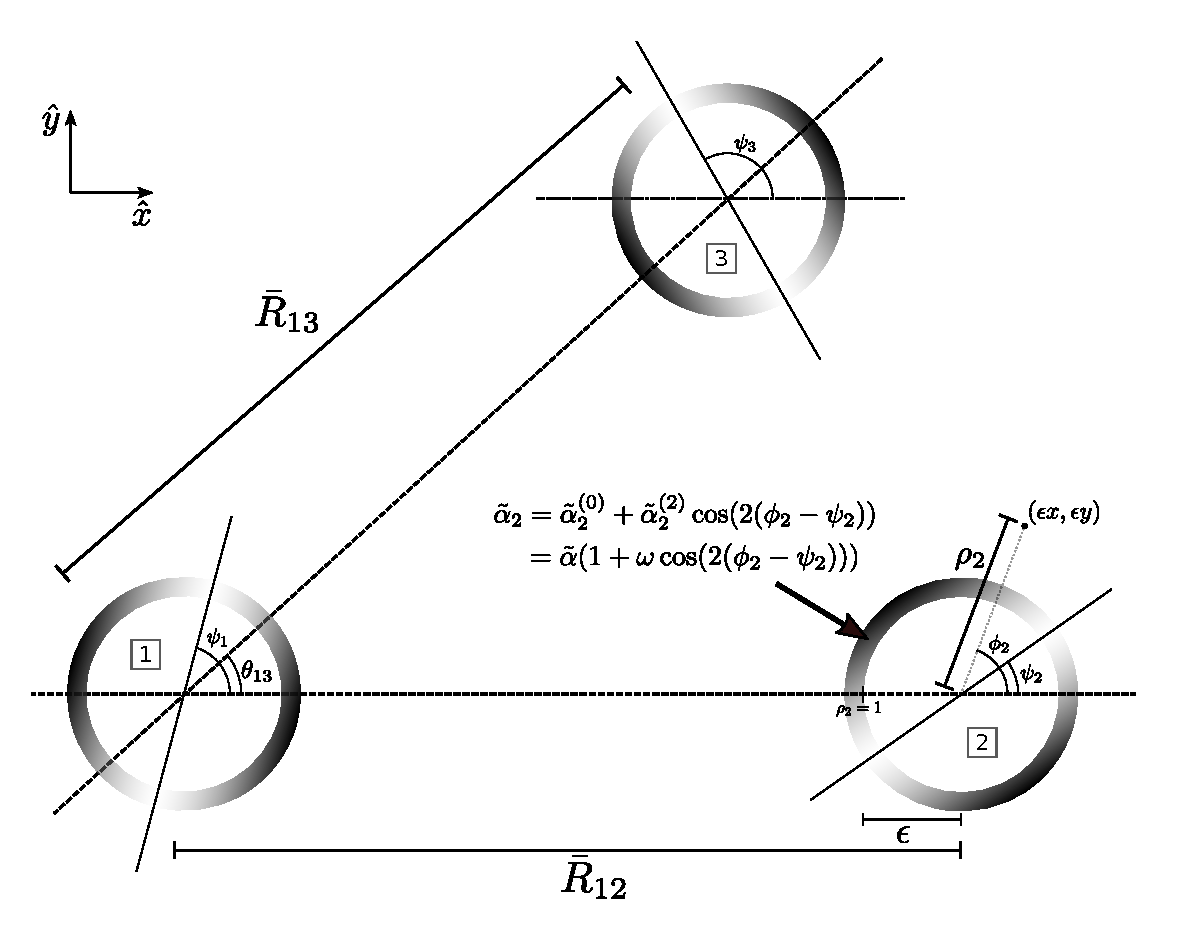
\includegraphics[width=12cm]{figures/3-elastic-figs/setup.pdf}
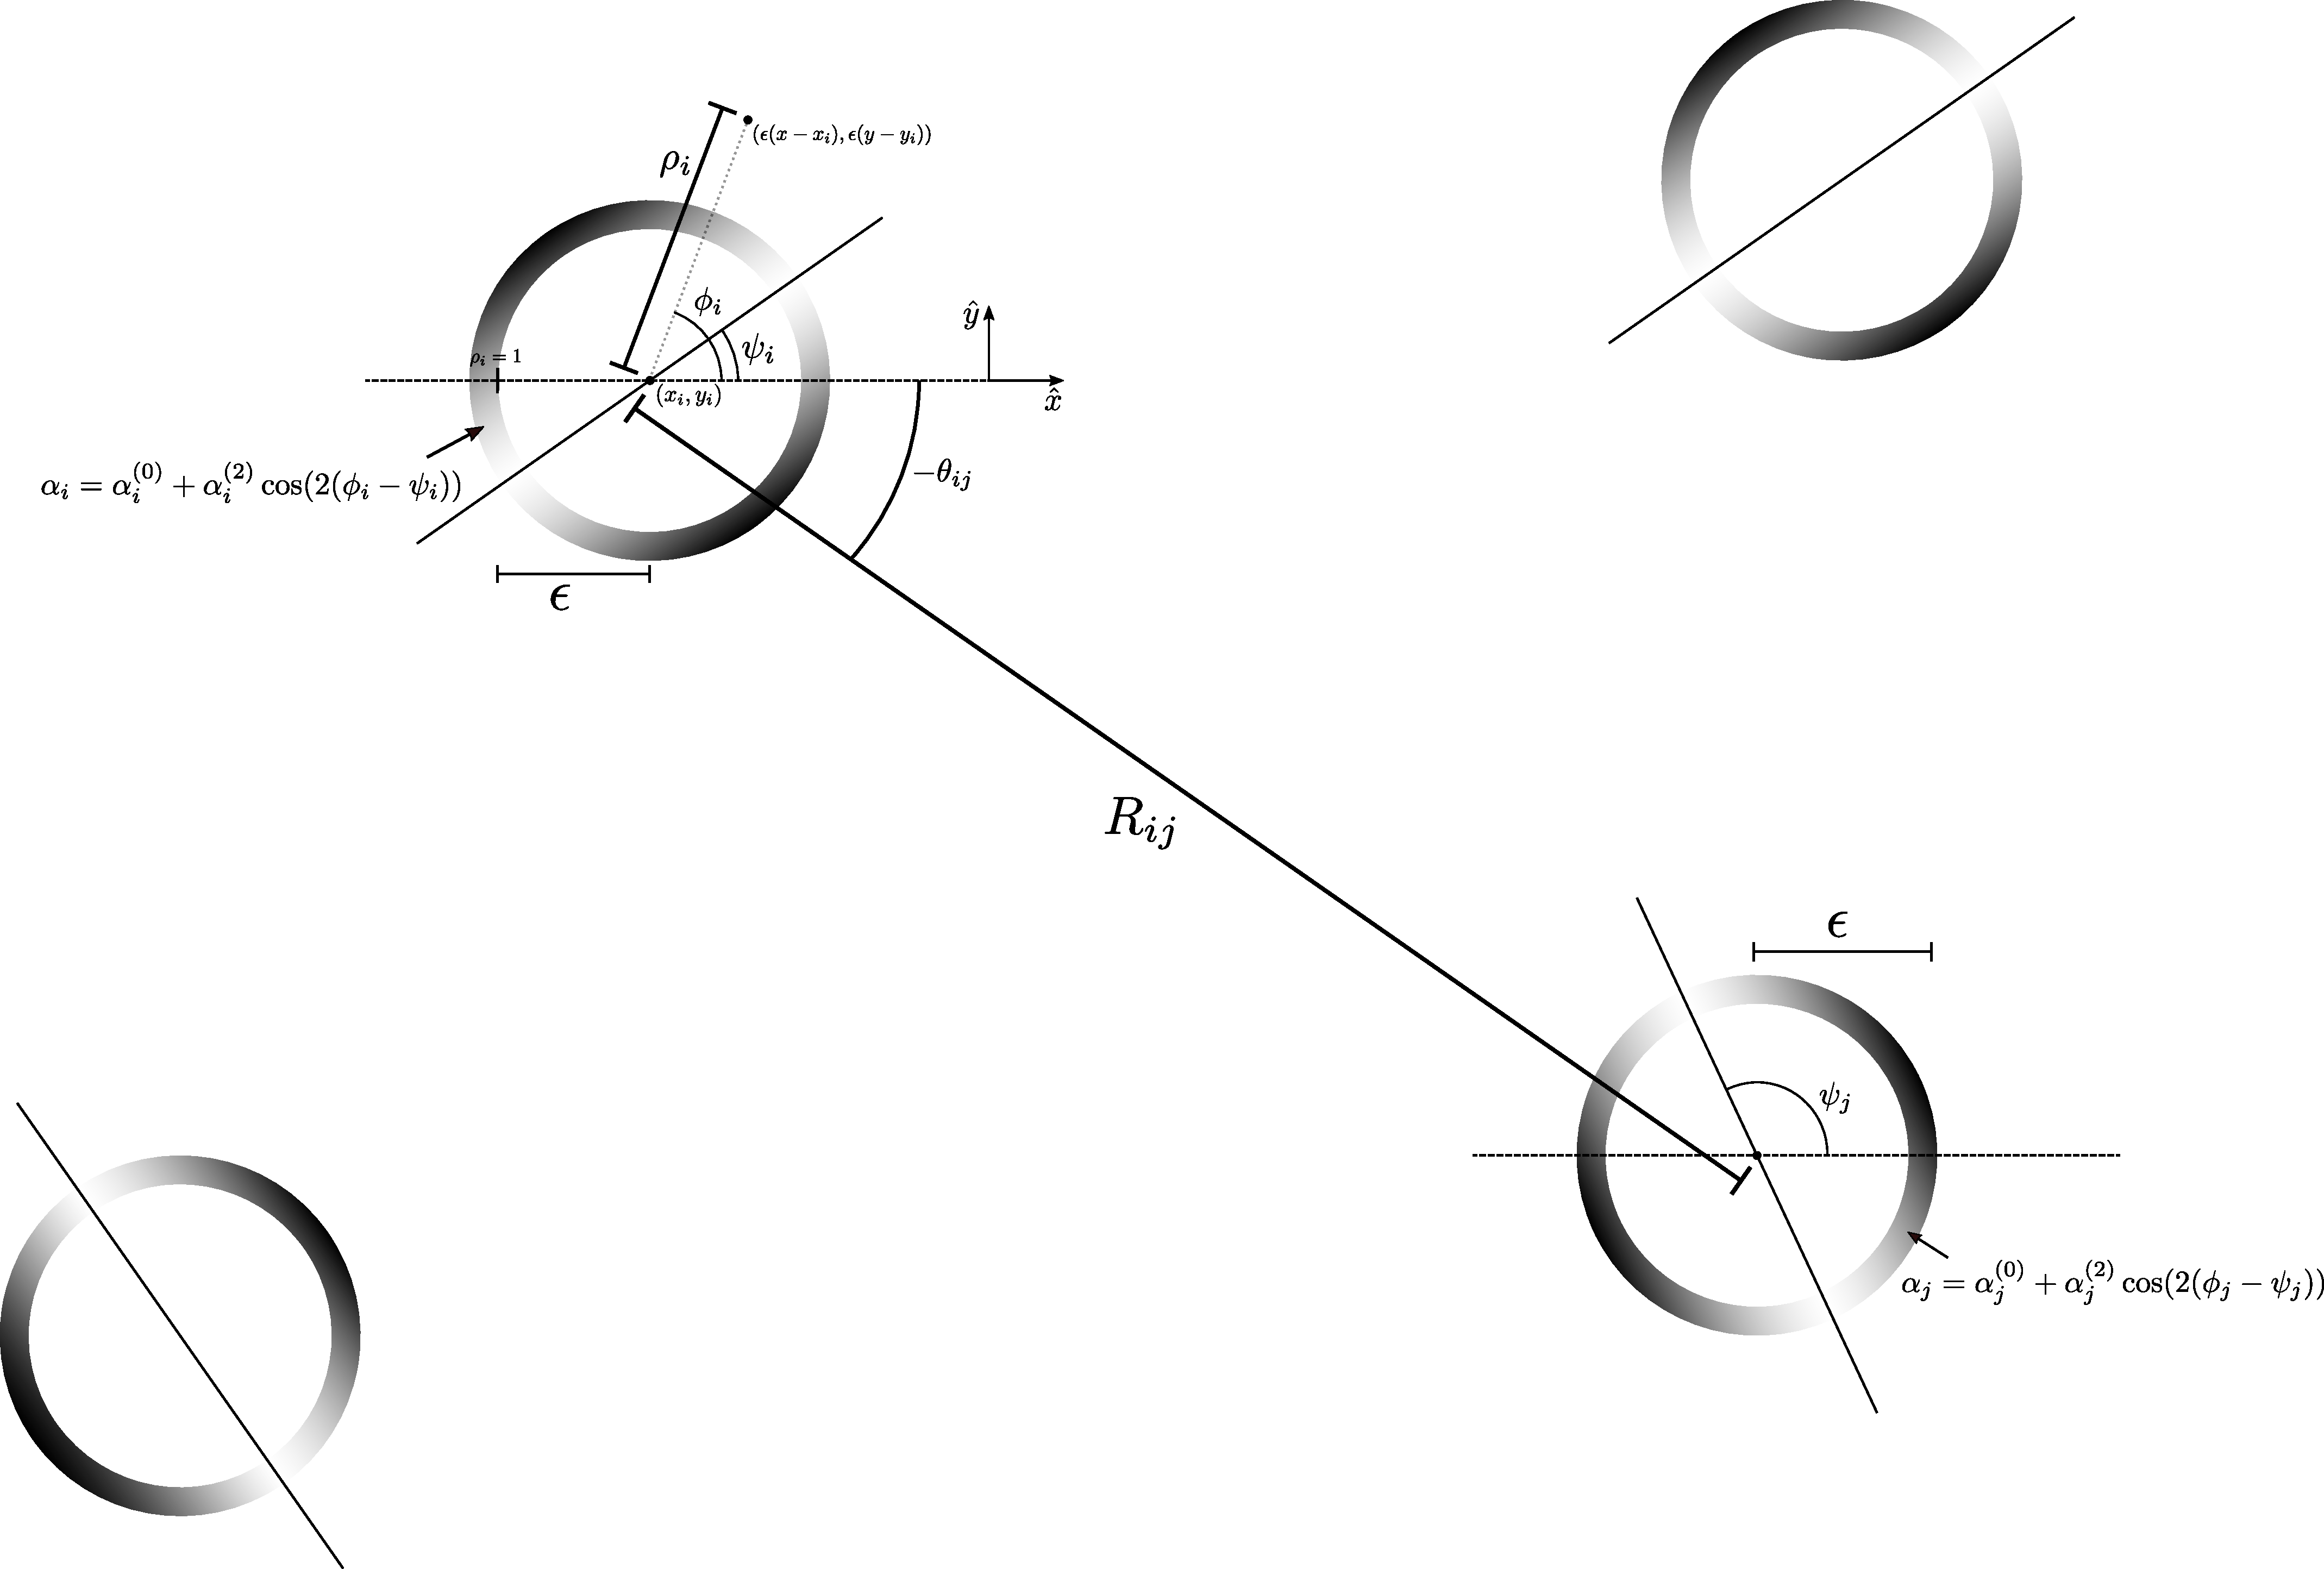
\includegraphics[width=12cm]{figures/3-elastic-figs/boundary_shade.pdf}
\caption{Parameterisation of the membrane elastic problem. The example shows the distribution of four inclusions where the inner coordinate system around the $i\text{th}$ inclusions is shown and the parameters describing the relative location of the $j\text{th}$ inlcusion are also shown. All angles are measured clockwise from the x-axis.}
\label{fig:setup}
\end{figure}

The inner region around the $i^{\text{th}}$ inclusion is described in local coordinates $(\rho_i, \phi_i)$, where the membrane height is $h_i(\rho_i, \phi_i)$ and the inclusion is a disc of radius 1. We expand the membrane height and the parameters describing the posture of the inclusion in the system in integer powers of $\epsilon$, for example, $h_i = h_i^{(0)}+\epsilon h_i^{(1)}+\epsilon^2 h_i^{(2)} + \cdots$ and $\beta_{i1} = \beta_{i1}^{(0)}+\epsilon \beta_{i1}^{(1)}+\epsilon^2 \beta_{i1}^{(2)} + \cdots$. In the inner coordinates, the shape equation (\ref{eq:shape_eq}) becomes
\begin{equation}
    \nabla^4_i h_i - \epsilon^2\mu^{-2}\nabla^{2}_i h_i = 0.
\end{equation}
where the subscript on the gradient operator indicates the coordinate system. This equation, along with the inclusion boundary conditions, must be satisfied at every order. The membrane shape in the outer region is given by $h_o(x, y)$, which we also expand in powers of $\epsilon$, and the inclusions appear as point singularities as $\epsilon\rightarrow0$.

\notyet{The inner region around the $i^{\text{th}}$ inclusion is described by the local coordinates $(\rho_i, \phi_i)$ and the membrane height in this region is $h_i(\rho_i, \phi_i)$ and the inclusion is a disc of radius $1$ in the inner coordinates. The membrane shape in the outer region is given by $h_o(x, y)$ and the inclusions appear as point singularities as $\epsilon\rightarrow0$. We expand the membrane height and parameters describing the posture of the inclusion in the system in integer powers of $\epsilon$, for example, $h_o = h_o^{(0)}+\epsilon h_o^{(1)}+\epsilon^2 h_o^{(2)} + \cdots$ and $\beta_{i1} = \beta_{i1}^{(0)}+\epsilon \beta_{i1}^{(1)}+\epsilon^2 \beta_{i1}^{(2)} + \cdots$. In the inner coordinates, the shape equation (\ref{eq:shape_eq}) becomes
\begin{equation}
    \nabla^4_i h_i - \epsilon^2\mu^{-2}\nabla^{2}_i h_i = 0.
\end{equation}
where the subscript on the gradient operator indicates the coordinate system. This equation, along with the inclusion boundary conditions, must be satisfied at every order.}

\notyet{\todo{need to have in here about the boundary and the tilt being a first order correction due to the radius epsilon term no?}}

\subsection{Matching}
At leading order the inner solution must satisfy
\begin{align}
    &\nabla_i^{4}h_i^{(0)}=0,  \\
    &h_i^{(0)}\biggr\rvert_{\rho_i=1}=\gamma_i^{(0)}, \\
    &\frac{\partial h_i^{(0)}}{\partial \rho_i}\biggr\rvert_{\rho_i=1}=\alpha_i^{(0)}+\alpha_i^{(2)}\cos(2\phi_i-2\psi_i).
\end{align}
\notyet{\todo{and the appropriate force balance conditions.}} In two-dimensional polar coordinates the biharmonic equation can be solved by separation of variables to obtain the so called  Michell solution. The boundary conditions only allow solutions with the monopole and quadrupole angular dependence, giving
\begin{equation}
    \begin{split}
    h_i^{(0)} &= \gamma_i^{(0)} + \alpha_i^{(0)}\log\rho_i + \frac{\alpha_i^{(2)}\cos 2\psi_i}{2}\cos 2\phi_i + \frac{\alpha_i^{(2)}\sin 2\psi_i}{2}\sin 2\phi_i \\
    &-\frac{\alpha_i^{(2)}\cos 2\psi_i}{2}\frac{\cos 2\phi_i}{\rho_i^2} - \frac{\alpha_i^{(2)}\sin 2\psi_i}{2}\frac{\sin 2\phi_i}{\rho_i^2}.
    \end{split}
\end{equation}
In the outer region, the shape equation for $h_o$ is the same at every order. For example, the leading order is
\begin{equation}
    \nabla^{4}h_o^{(0)}-\mu^{-2}\nabla^{2}h_o^{(0)}=0.  
\end{equation}
Around each inclusion the membrane approaches a singularity, which must match with the inner solution. This solution that matches and decays at infinity is given by
\begin{equation}
    h_o^{(0)} = c_0 + \sum_i \left( c_{1i} K_0(r_i/\mu) + c_{2i} \cos(2\phi_i-2\psi_i)\left(\frac{4\mu^{2}}{r_i^2} - 2 K_2(r_i/\mu)\right) \right),
\end{equation}
where $r_i = ((x_ - x_i)^2+(y - y_i)^2)^{1/2}$ and $\phi_i = \tan^{-1}((y - y_i)/(x - x_i))$. Expanding in inner variables about inclusion $i$ gives
\begin{alignat}{2}
        h_o^{(0)} &= c_0\; - &&c_{1i}(\gamma + \log(\epsilon\rho_{i}/2\mu))+\frac{c_{1i}}{4}(1-\gamma + \log 2 - \log \epsilon\rho_{i}/\mu)\frac{\epsilon^2 \rho_{i}^2}{\mu^2} \notag\\
        &+ c_{2i}\cos&&(2\phi_i-2\psi_i)\left( 1 + \frac{\epsilon^2\rho_{i}^2\log(\epsilon\rho_{i}/2\mu)}{4\mu^2} + \frac{\epsilon^2\rho_{i}^2(4\gamma - 3)}{16\mu^2}\right)\notag\\
        &+\mathlarger{\mathlarger{\sum}}_{j\neq i}&&\Bigg\{c_{1j}\Bigg[K_0\left(\frac{R_{ij}}{\mu}\right) + \frac{K_1\left(\frac{R_{ij}}{\mu}\right)}{\mu}\epsilon\rho_{i}\cos(\phi_i-\theta_{ij}) + \frac{K_0\left(\frac{R_{ij}}{\mu}\right)}{{2\mu^2}}\epsilon^2\rho_{i}^2\cos^2(\phi_i-\theta_{ij})\notag\\
        & &&+ \frac{K_1\left(\frac{R_{ij}}{\mu}\right)}{2\mu R_{ij}}\cos(2\phi_i-2\theta_{ij})\epsilon^2\rho_{i}^2\Bigg] \notag\\
        & &&+ c_{2j}\Bigg[\cos(2\psi_j-2\theta_{ij})\Bigg(f\left(\frac{R_{ij}}{\mu}\right) - \frac{\epsilon\rho_{i}\cos(\theta_{ij}-\phi_i)f'\left(\frac{R_{ij}}{\mu}\right)}{\mu} \notag\\
        & &&+ \epsilon^2\rho_{i}^2\bigg(-\frac{2f\left(\frac{R_{ij}}{\mu}\right)\sin^2(\phi_i-\theta_{ij})}{R_{ij}^2}+\frac{\sin^2(\phi_i-\theta_{ij})f'\left(\frac{R_{ij}}{\mu}\right)}{2\mu R_{ij}} + \frac{\cos^2(\phi_i-\theta_{ij})f''\left(\frac{R_{ij}}{\mu}\right)}{2\mu^2}\bigg)\Bigg)\notag\\
        & &&+ \sin(2\psi_j-2\theta_{ij})\Bigg(-\frac{2\epsilon\rho_{i} f\left(\frac{R_{ij}}{\mu}\right)\sin(\phi_i-\theta_{ij})}{R_{ij}} \notag\\
        & &&+ \epsilon^2\rho_{i}^2\bigg(-\frac{2\cos(\phi_i-\theta_{ij})f\left(\frac{R_{ij}}{\mu}\right)\sin(\phi_i-\theta_{ij})}{ R_{ij}^2} + \frac{2\cos(\phi_i-\theta_{ij})\sin(\phi_i-\theta_{ij})f'\left(\frac{R_{ij}}{\mu}\right)}{R_{ij}\mu}\bigg)\Bigg)\Bigg]\Bigg\} + O(\epsilon^3), %no \notag to number the equation
    \label{eq:leadingoutersecondinner}
\end{alignat}
which matches the leading order inner solutions to give
\begin{equation}
    c_{1i} = -\alpha_{i}^{0}, \quad c_{2i} = \frac{\alpha_{i}^{2}}{2},
\end{equation}
and
\begin{equation}
    \gamma_i^{(0)} = c_0 - c_{1i}\left(\log\frac{\epsilon}{2\mu}+\gamma\right) +\mathlarger{\sum}_{i\neq j}\left\{c_{1j}K_0(R_{ij}/\mu) +c_{2j}\cos(2\psi_j)\left(\frac{4\mu^2}{R_{ij}^2}- 2K_{2}(R_{ij}/\mu)\right)\right\}.
\end{equation}
At first order, the inner equation is
\begin{align}
    &\nabla_i^{4}h_i^{(1)}=0, \label{inner1order}\\ &h_i^{(1)}\biggr\rvert_{\rho_i=1}=\gamma_i^{(1)}+\beta^{(0)}_{i1}\cos(\phi_i)+\beta^{(0)}_{i2}\sin(\phi_i), \label{inner1orderBCval}\\
    &\frac{\partial h_i^{(1)}}{\partial \rho_i}\biggr\rvert_{\rho_i=1}=\beta^{(0)}_{i1}\cos(\phi_i)+\beta^{(0)}_{i2}\sin(\phi_i).\label{inner1orderBCderriv}
\end{align}
Additionally, as $\rho_1\to\infty$ the solution must match with the first order terms in equation (\ref{eq:leadingoutersecondinner}) and so 
\begin{equation}
\begin{split}
    h_i^{(1)}\biggr\rvert_{\rho_i\to\infty} \sim \mathlarger{\mathlarger{\sum}}_{j \neq i} \Bigg\{ &\rho_i \cos (\phi_i) \Bigg(\frac{c_{1j} \cos (\theta_{ij}) \left( K_1\left(\frac{R_{ij}}{\mu }\right) - c_{2j} \cos (2 \psi_j-2 \theta_{ij} ) f'\left(\frac{R_{ij}}{\mu }\right)\right)}{\mu}\\
    &+\frac{2 c_{2j} \sin (\theta_{ij} ) f\left(\frac{R_{ij}}{\mu }\right) \sin (2 \psi_j-2 \theta_{ij} )}{R_{ij}}\Bigg) \\
    &+\rho_i  \sin (\phi_i) \Bigg(\frac{\sin (\theta_{ij} ) \left(c_{1j} K_1\left(\frac{R_{ij}}{\mu }\right)-c_{2j} \cos (2 \psi_j-2 \theta_{ij} ) f'\left(\frac{R_{ij}}{\mu }\right)\right)}{\mu } \\
    &-\frac{2 c_{2j} \cos (\theta_{ij} ) f\left(\frac{R_{ij}}{\mu }\right) \sin (2 \psi_j-2 \theta_{ij} )}{R_{ij}}\Bigg)\Bigg\}.
\end{split}
\end{equation}
The solution to (\ref{inner1order}) with the correct limiting behaviour is
\begin{equation}
    h_i^{(1)} = \gamma_i^{(1)}+\beta^{(0)}_{i1} \rho_i \cos(\phi_i)+\beta^{(0)}_{i2} \rho_i \sin(\phi_i)
\end{equation}
where the matching gives
\begin{equation}
\begin{split}
    \beta^{(0)}_{i1} = \mathlarger{\sum}_{j \neq i}\; &\frac{c_{1j} K_1\left(\frac{R_{ij}}{\mu}\right)\cos (\theta_{ij})}{\mu}-\frac{c_{2j} \cos (2 \psi_j-2\theta_{ij})\cos (\theta_{ij}) f'\left(\frac{R_{ij}}{\mu }\right)}{\mu}\\
    &+\frac{2 c_{2j} \sin (\theta_{ij}) f\left(\frac{R_{ij}}{\mu }\right) \sin (2\psi_j-2 \theta_{ij})}{R_{ij}}, \\
    \beta^{(0)}_{i2} = \mathlarger{\sum}_{j \neq i}\; &\frac{c_{1j} K_1\left(\frac{R_{ij}}{\mu}\right)\sin (\theta_{ij})}{\mu}-\frac{c_{2j} \cos (2 \psi_j-2\theta_{ij})\sin (\theta_{ij}) f'\left(\frac{R_{ij}}{\mu }\right)}{\mu}\\
    &-\frac{2 c_{2j} \cos (\theta_{ij}) f\left(\frac{R_{ij}}{\mu }\right) \sin (2\psi_j-2 \theta_{ij})}{R_{ij}}.
\end{split}
\end{equation}
Note the difference of sign in the term $\sim \sin (2\psi_j-2 \theta_{ij})$ between $\beta^{(0)}_{i1}$ and $\beta^{(0)}_{i2}$.
\notyet{This is due to the symmetry of the This can be understood by considering a change of coordinate system, for example changing the sign of one axis (such that any angle $\sigma \rightarrow -\sigma$), or a by a rotation of $\pi/2$ ($\sigma \rightarrow \sigma - \pi/2$). Under a rotation of $\pi/2$, we would expect the coefficients of the terms $\sim\sin\phi_i$ and $\sim\cos\phi_i$ to swap and so $\beta^{(0)}_{i1} \rightarrow \beta^{(0)}_{i2}$ and $\beta^{(0)}_{i2} \rightarrow \beta^{(0)}_{i1}$. The change of sign comes since the terms that go like cosine change sign, whereas those that go like sine do not. As such any term containing an odd number of cosines should change sign between the two coefficients, which here is only the term $\sim \sin (2\psi_j-2 \theta_{ij})$.}
% and at second order the Laplacian of the leading order solution is also included
% \begin{align}
%     &\nabla_i^{4}h_i^{(2)}-\mu^{-2}\nabla^{2}_i h_i^{(0)}=0,  \\
%     &h_i^{(2)}\biggr\rvert_{\rho_i=1}=\gamma_i^{(2)}+\beta^{(1)}_{i1}\cos(\phi_i)+\beta^{(1)}_{i2}\sin(\phi_i), \\
%     &\frac{\partial h_i^{(2)}}{\partial \rho_i}\biggr\rvert_{\rho_i=1}=\beta^{(1)}_{i1}\cos(\phi_i)+\beta_{i2}\sin(\phi_i). 
% \end{align}

% The first order outer solution satisfies
% \begin{equation}
%     \nabla^{4}h_o^{(1)}-\mu^{-2}\nabla^{2}h_o^{(1)}=0
% \end{equation}
% and must match with eqaution (ref), giving
% \begin{equation}
%     h_o^{(1)} = \gamma_i^{(1)}.
% \end{equation}
% Since this matching can be done around any inclusion, this relationship holds for all inclusions.

For the second order inner solution we have
\begin{align}
    &\nabla_i^{4}h_i^{(2)}=\nabla_i^{2}h_i^{(0)}=-\frac{2\alpha^{(2)}_{1}\cos(2\phi_i-2\psi_i)}{\mu^2\rho^2}, \label{secondinner}\\
    &h_i^{(2)}\biggr\rvert_{\rho_i=1}=\gamma_i^{(2)}+\beta^{(1)}_{i1}\cos(\phi_i)+\beta^{(1)}_{i2}\sin(\phi_i), \\
    &\frac{\partial h_i^{(2)}}{\partial \rho_i}\biggr\rvert_{\rho_i=1}=\beta^{(1)}_{i1}\cos(\phi_i)+\beta^{(1)}_{i2}\sin(\phi_i).
\end{align}
and from matching with the second order terms in equation (\ref{eq:leadingoutersecondinner}) we find that
\begin{equation}
    \begin{split}  
        h_i^{(2)}\biggr\rvert_{\rho_i\to\infty} \sim& -\rho_{i}^2 \frac{\alpha_{i}^{(0)}}{4\mu^2}(1-\gamma - \log \epsilon - \log \rho_{i}/2\mu) \\
        &+ \alpha_{i}^{(2)}\cos(2\phi_i-2\psi_i)\left(\frac{\epsilon^2\rho_{i}^2\log(\epsilon\rho_{1}/2\mu)}{8\mu^2} + \frac{\epsilon^2\rho_{i}^2(4\gamma - 3)}{32\mu^2}\right)\\
        +\sum_{j}\Bigg\{\rho_i^2\Bigg[-&\alpha_{j}^{(0)}\frac{K_0\left(\frac{R_{ij}}{\mu}\right)}{{4\mu^2}}+\alpha_{j}^{(2)}\cos(2\theta_{ij}-2\psi_j)\left(\frac{-f\left(\frac{R_{ij}}{\mu}\right)}{2R_{ij}^2}+\frac{f'\left(\frac{R_{ij}}{\mu}\right)}{8 \mu R_{ij}}+\frac{f''\left(\frac{R_{ij}}{\mu}\right)}{8 \mu^2}\right)\Bigg]\\
        +\cos2\phi_i\rho_i^2&\Bigg[-\alpha_{j}^{(0)}\cos2\theta_{ij}\frac{R_{ij}K_0\left(\frac{R_{ij}}{\mu}\right)+2\mu K_1\left(\frac{R_{ij}}{\mu}\right)}{{4\mu^2}R_{ij}}\\
        &+\alpha_{j}^{(2)}\sin(2\theta_{ij})\sin(2\psi_j-2\theta_{ij})\left(\frac{f\left(\frac{R_{ij}}{\mu}\right)}{2R_{ij}^2}-\frac{f'\left(\frac{R_{ij}}{\mu}\right)}{2\mu R_{ij}}\right)\\
        & +\alpha_{j}^{(2)}\cos(2\theta_{ij})\cos(2\psi_j-2\theta_{ij})\left(\frac{f\left(\frac{R_{ij}}{\mu}\right)}{2 R_{ij}^2}-\frac{f'\left(\frac{R_{ij}}{\mu}\right)}{8 \mu R_{ij}}+\frac{f''\left(\frac{R_{ij}}{\mu}\right)}{8 \mu^2}\right)\Bigg]\\
        +\sin2\phi_i\rho_i^2&\Bigg[-\alpha_{j}^{(0)}\sin2\theta_{ij}\frac{R_{ij}K_0\left(\frac{R_{ij}}{\mu}\right)+2\mu K_1\left(\frac{R_{ij}}{\mu}\right)}{{4\mu^2}R_{ij}}\\
        &+ \alpha_{j}^{(2)}\sin(2\theta_{ij})\cos(2\psi_j-2\theta_{ij})\left(\frac{f\left(\frac{R_{ij}}{\mu}\right)}{2R_{ij}^2}-\frac{f'\left(\frac{R_{ij}}{\mu}\right)}{8 \mu R_{ij}}+\frac{f''\left(\frac{R_{ij}}{\mu}\right)}{8 \mu^2}\right)\\
        & +\alpha_{j}^{(2)}\cos(2\theta_{ij})\sin(2\psi_j-2\theta_{ij})\left(\frac{f\left(\frac{R_{ij}}{\mu}\right)}{2 R_{ij}^2}-\frac{f'\left(\frac{R_{ij}}{\mu}\right)}{2 \mu R_{ij}}\right)\Bigg]\Bigg\}\\
    \end{split}
\end{equation}
where we have used that as $r \rightarrow 0$, $f \sim 1 + \frac{r^2\log(r/2)}{4} + \frac{4\gamma-3 r^2}{16}$. Identifying the terms that depend on the inner coordinate system we write this last expression as
\begin{equation}
    \begin{split}
        h_i^{(2)}\biggr\rvert_{\rho_i\to\infty} = & M_C \rho_i^2 \cos(2\phi_i) + M_S \rho_i^2 \sin(2\phi_i) + M_0\rho_i^2 + M_1\rho_i^2\log\rho_i \\
        +& c_{2i}\cos(2\phi_i-2\psi_i)\left(\frac{\rho_{i}^2\log(\epsilon\rho_{i}/2\mu)}{4\mu^2} + \frac{\rho_{i}^2(4\gamma - 3)}{16\mu^2}\right).
    \end{split}
    \label{secondinnerBCfar}
\end{equation}
The solution is
\begin{equation}
    \begin{split}
        h_i^{(2)}\biggr\rvert_{\rho_i\to\infty} \sim &  \gamma^{(2)} + c_{2i}\cos(2\phi_i-2\psi_i)\left(\frac{\rho_{i}^2\log(\epsilon\rho_{i}/2\mu)}{4\mu^2} + \frac{\rho_{i}^2(4\gamma - 3)}{16\mu^2}\right) \\
        +& \mathcal{M}_C\left(\rho_i^2-2+\frac{1}{\rho_i^2}\right)\cos(2\phi) + \mathcal{M}_S\left(\rho_i^2-2+\frac{1}{\rho_i^2}\right)\sin(2\phi)\\
        +& M_0(-1+\rho_1^2-2\ln{\rho_1})+ M_1(\rho_1^2\ln{\rho_1}-\ln{\rho_1}),
    \end{split}
\end{equation}
where we have considered each angular mode separately. Terms that go like $\sim\cos(n\phi_i)$ and $\sim\sin(n\phi_i)$ with $n \geq 3$ do not appear in the solution to the shape equation as they cannot satisfy the matching and boundary conditions. When $n=1$, the solution would be $(A_1 (\rho_i-\rho_i^{-2}-2\rho_i\log(\rho_i))+\beta_{i1}^{(1)}\rho_i\log(\rho_i))\cos(\phi_i)$ and similarly for $\sin(\phi_i)$. However, the terms that are linear in $\rho_i$ would appear at first order and would therefore be included in $h_i^{(1)}$. Since these terms are not in equation (\todo{ref}) we find that $\beta_{i1}^{(1)}=\beta_{i2}^{(1)}=0$ and so there is no $n=1$ contribution to $h_i^{(2)}$. Writing out the full solution gives
\notyet{
The particular solution to (\ref{secondinner}) is $\frac{\rho_i^2\alpha_i^{(2)}}{8\mu^2}\cos(2\phi_i-2\psi_i)\log\rho_i$ and terms with this angular periodicity and offset must vanish at the boundary and farfield. This is solved by $\frac{\alpha_i^{(2)}}{16\mu^2}\cos(2\phi_i-2\psi_i)(\rho_i^2(2\gamma - 3/2) + (1/\rho_i^2)(2\gamma - 1/2 + 2\log{(\epsilon/2\mu)}) + (2 - 4\gamma - 4\log{(\epsilon/2\mu)})$.

To match with (\ref{secondinnerBCfar}) we consider each angular mode ($\sim\cos(n\phi_i)$ and $\sim\sin(n\phi_i)$) separately.  The $n=0$ mode goes like $M_0\rho_1^2+M_1\rho_1^2\log\rho_1$ as $\rho_1 \rightarrow \infty$, and is equal to $\gamma^{(2)}$ at the boundary with vanishing derivatives. This is solved by $\gamma^{(2)} + M_0(-1+\rho_1^2-2\ln{\rho_1})+ M_1(\rho_1^2\ln{\rho_1}-\ln{\rho_1})$. When $n=1$, the solution would be $(A_1 (\rho_i-\rho_i^{-2}-2\rho_i\log(\rho_i))+\beta_{i1}^{(1)}\rho_i\log(\rho_i))\cos(\phi_i)$ and similarly for $\sin(\phi_i)$. However, the terms that are linear in $\rho_i$ would appear at first order and would therefore be included in $h_i^{(1)}$. Since these terms are not in equation (\todo{ref}) we find that $\beta_{i1}^{(1)}=\beta_{i2}^{(1)}=0$ and so there is no $n=1$ mode in $h_i^{(2)}$.

The $n=2$ terms vanish at the boundary, but appear in the matching condition.
When $n=2$ the solution is $\sim\mathcal{M}_C(\rho_i^2-2+\frac{1}{\rho_i^2})\cos(2\phi)$ and $\sim\mathcal{M}_S(\rho_i^2-2+\frac{1}{\rho_i^2})\sin(2\phi)$, which vanishes at the boundary and matches in the far field.

Terms with angular periodicity $n \geq 3$ must be equal to zero everywhere as they do not appear in (\ref{secondinner}), the matching, or the boundary conditions.

We can solve (\ref{secondinner}) for $h_i^{(2)}$ by considering each of these terms separately. The particular solution is $\frac{\rho_i^2\alpha_i^{(2)}}{8\mu^2}\cos(2\phi_i-2\psi_i)\log\rho_i$ Terms with this angular periodicity and offset must vanish at the boundary along with their derivatives and must have the correct farfield matching. The terms that solve the homogeneous equation and give the appropriate contributions to satisfy the boundary conditions are $\frac{\alpha_i^{(2)}}{16\mu^2}\cos(2\phi_i-2\psi_i)(\rho_i^2(2\gamma - 3/2) + (1/\rho_i^2)(2\gamma - 1/2 + 2\log{(\epsilon/2\mu)}) + (2 - 4\gamma - 4\log{(\epsilon/2\mu)})$.

Terms that go like $\sim\cos(n\phi_i)$ and $\sim\sin(n\phi_i)$ with angular periodicity $n \geq 3$ must be equal to zero everywhere as they do not appear in the matching or boundary conditions. When $n=1$, the solution would be $(A_1 (\rho_i-\rho_i^{-2}-2\rho_i\log(\rho_i))+\beta_{i1}^{(1)}\rho_i\log(\rho_i))\cos(\phi_i)$ and similarly for $(A_1 (\rho_i-\rho_i^{-2}-2\rho_i\log(\rho_i))+\beta_{i2}^{(1)}\rho_i\log(\rho_i))\sin(\phi_i)$. However, the terms that are linear in $\rho_i$ would appear at first order and would be included in $h_i^{(1)}$. Since these terms are not in equation (\todo{ref}) we find that $\beta_{i1}^{(1)}=\beta_{i2}^{(1)}=0$.

Terms with angular periodicity $n=2$ vanish at the boundary, but appear in the matching condition. The solution to the biharmonic equation with these conditions is $\sim\mathcal{M}_C(\rho_i^2-2+\frac{1}{\rho_i^2})\cos(2\phi)$ and $\sim\mathcal{M}_S(\rho_i^2-2+\frac{1}{\rho_i^2})\sin(2\phi)$. The $n=0$ mode goes like $M_0\rho_1^2+M_1\rho_1^2\log\rho_1$ as $\rho_1 \rightarrow \infty$, and is equal to $\gamma^{(2)}$ at the boundary with vanishing derivatives. This is solved by $\gamma^{(2)} + M_0(-1+\rho_1^2-2\ln{\rho_1})+ M_1(\rho_1^2\ln{\rho_1}-\ln{\rho_1})$. The second order inner solution with coefficients determined by matching is therefore}
\begin{alignat}{3}
    h_i^{(2)} &=\;&& \gamma^{(2)} + && \frac{\left(-\alpha_{i}^{(0)}\right)}{4\mu^2}  \left(\rho_{i}^2\log \rho_{i} - \log \rho_{i}\right) \notag\\
    % + \left(\frac{\alpha_{i}^{(2)}}{2}\right)\cos(2\phi_i-2\psi_i) \left(\frac{\epsilon^2\rho_{i}^2\log(\epsilon\rho_{1}/2\mu)}{4\mu^2} + \frac{\epsilon^2\rho_{i}^2(4\gamma - 3)}{16\mu^2}\right)
    &\;+&&\frac{\alpha_i^{(2)}}{16\mu^2}&&\cos(2\phi_1-2\psi)\left(\rho_1^2(2\gamma - 3/2) + \frac{2\gamma - 1/2 + 2\log{\left(\frac{\epsilon}{2\mu}\right)}}{\rho_i^2} + 2 - 4\gamma - 4\log{\left(\frac{\epsilon}{2\mu}\right)}\right) \notag\\
    &\;+&& \big(-1 &&+ \rho_{i}^2 + 2\log\rho_{i}\big)\Bigg(\frac{\left(-\alpha_{i}^{(0)}\right)}{4\mu^2}(1-\gamma - \log (\epsilon/2\mu)) \notag\\
    & && &&+ \sum_{j \neq i}\Bigg\{\left(-\alpha_{j}^{(0)}\right)\frac{K_0\left(\frac{R_{ij}}{\mu}\right)}{{4\mu^2}}+\left(\frac{\alpha_{j}^{(2)}}{2}\right)\cos(2\theta_{ij}-2\psi_j)\left(\frac{-f\left(\frac{R_{ij}}{\mu}\right)}{R_{ij}^2}+\frac{f'\left(\frac{R_{ij}}{\mu}\right)}{4 \mu R_{ij}}+\frac{f''\left(\frac{R_{ij}}{\mu}\right)}{4 \mu^2}\right)\Bigg\}\Bigg) \notag\\
    &\;+&& \sum_{j \neq i}&& \Bigg\{\cos2\phi_i \left(\rho_i^2-2+\frac{1}{\rho_i^2}\right) \Bigg[\left(-\alpha_{j}^{(0)}\right)\cos2\theta_{ij}\frac{R_{ij}K_0\left(\frac{R_{ij}}{\mu}\right)+2\mu K_1\left(\frac{R_{ij}}{\mu}\right)}{{4\mu^2}R_{ij}} \notag\\
    & && &&+\left(\frac{\alpha_{j}^{(2)}}{2}\right)\sin(2\theta_{ij})\sin(2\psi_j-2\theta_{ij})\left(\frac{f\left(\frac{R_{ij}}{\mu}\right)}{R_{ij}^2}-\frac{f'\left(\frac{R_{ij}}{\mu}\right)}{\mu R_{ij}}\right) \notag\\
    & && &&+\left(\frac{\alpha_{j}^{(2)}}{2}\right)\cos(2\theta_{ij})\cos(2\psi_j-2\theta_{ij})\left(\frac{f\left(\frac{R_{ij}}{\mu}\right)}{R_{ij}^2}-\frac{f'\left(\frac{R_{ij}}{\mu}\right)}{4 \mu R_{ij}}+\frac{f''\left(\frac{R_{ij}}{\mu}\right)}{4 \mu^2}\right)\Bigg] \notag\\
    & && \quad + &&\sin2\phi_i\left(\rho_i^2-2+\frac{1}{\rho_i^2}\right)\Bigg[\left(-\alpha_{j}^{(0)}\right)\sin2\theta_{ij}\frac{R_{ij}K_0\left(\frac{R_{ij}}{\mu}\right)+2\mu K_1\left(\frac{R_{ij}}{\mu}\right)}{{4\mu^2}R_{ij}} \notag\\
    & && &&+ \left(\frac{\alpha_{j}^{(2)}}{2}\right)\sin(2\theta_{ij})\cos(2\psi_j-2\theta_{ij})\left(\frac{f\left(\frac{R_{ij}}{\mu}\right)}{R_{ij}^2}-\frac{f'\left(\frac{R_{ij}}{\mu}\right)}{4 \mu R_{ij}}+\frac{f''\left(\frac{R_{ij}}{\mu}\right)}{4 \mu^2}\right) \notag\\
    & && &&+\left(\frac{\alpha_{j}^{(2)}}{2}\right)\cos(2\theta_{ij})\sin(2\psi_j-2\theta_{ij})\left(\frac{f\left(\frac{R_{ij}}{\mu}\right)}{R_{ij}^2}-\frac{f'\left(\frac{R_{ij}}{\mu}\right)}{\mu R_{ij}}\right)\Bigg]\Bigg\}.
\end{alignat}

This gives sufficient terms in the expansion of the height to calculate the deformation energy.

\subsection{Membrane Interaction Energy}

We can now use the shape of the membrane to find the energy of a given configuration of inclusions. The energy comes from evaluating (\ref{eq:efull}) which can be more easily calculated in this regime by integrating by parts, and evaluating the boundary terms as in equation (\ref{eq:eparts}). Since the membrane is flat at infinity ($\frac{\partial h}{\partial \rho_1} = 0$ as $\rho_1 \rightarrow \infty$) the integral is simply the integral around the edge of each inclusion which we calculate in the inner region.\notyet{This can be performed in the inner variables and using 
\begin{equation}
    \int_{\partial\Omega_i}\text{d}s \rightarrow \int_0^{2\pi} \epsilon\times \text{d}\phi_i|_{\rho_i=1},\quad
    \nabla = \frac{1}{\epsilon}\nabla_i,\quad \frac{\partial}{\partial n_i} = -\frac{1}{\epsilon}\frac{\partial}{\partial\rho_i}
\end{equation}
at each inclusion.} We consider this integral to first order in $\epsilon$ which gives the boundary energy term around the $i$th inclusion as
\begin{equation}
\begin{split}
    E_i &= \pi\left(\alpha_i^{(2)}\right)^2\left(\frac{1}{\epsilon} + \frac{\gamma}{\mu^2} + \frac{\log(\frac{\epsilon}{2\mu})}{\mu^2}\right) - \pi\left(\alpha_i^{(0)}\right)^2\left(\frac{\gamma}{2\mu^2} + \frac{\log(\frac{\epsilon}{2\mu})}{2\mu^2}\right) \\
    &\sum_{j\neq i}\Bigg[\frac{\pi \alpha_i^{(2)}\alpha_j^{(2)}}{2\mu^2}\left(\cos\left(4\theta_{ij}-2(\psi_i+\psi_j)\right)\left(\frac{-48\mu^4}{R_{ij}^4} + K_4\left(\frac{R_{ij}}{\mu}\right)\right) + \cos\left(2\psi_i-2\psi_j\right)K_0\left(\frac{R_{ij}}{\mu}\right)\right) \\
    &+ \frac{\pi  \alpha_i^{(0)} \alpha_j^{(0)}}{\mu ^2} K_0\left(\frac{R_{ij}}{\mu }\right) + \frac{\pi  \alpha_i^{(0)} \alpha_j^{(2)}}{\mu ^2} \cos (2\psi_j-2\theta_{ij}) K_2\left(\frac{R_{ij}}{\mu }\right) + \frac{\pi  \alpha_j^{(0)} \alpha_i^{(2)}}{\mu ^2} \cos (2\psi_i-2\theta_{ij}) K_2\left(\frac{R_{ij}}{\mu }\right)\Bigg],
    \end{split}
    \label{eq:E_inc_boundary}
\end{equation}
\todo{check pis etc and compare to one inclusion case} where we have substituted in the form of $f(x)$ and simplified the resulting expressions. The constant term before the sum is the energy deformation energy from one-inclusion and is identical to (\ref{eq:SingleModQuad}). The total membrane energy of a configuration is the sum of these boundary integrals, $E = \sum_{i}E_i$. The energy consists of a constant term for each inclusion that is independent of the inclusion configuration and the interaction term that for each inclusion runs over the sum of all other inclusions. We can rewrite this double sum as a sum over all unique pairs of inclusions. For each pair of inclusions, labelled $k$ and $l$, there will be a contribution to the energy when $i=k$ and $j=l$ and also when $i=l$ and $j=k$ and from the geometry of the system $R_{kl} = R_{lk}$ and $\theta_{kl} = \theta_{lk}+\pi$ (up to a shift of $2\pi$). Thus, the summand is unchanged under the exchange of these indices and both terms involving a unique pair of inclusions are the same. The interaction energy between a configuration of inclusions is therefore the pairwise sum of the two body interaction energy $E_2$
\begin{equation}
\begin{split}
    E_2(R_{12}, &\theta_{12}, \psi_1,  \psi_2) = \frac{\pi\alpha_1^{(2)}\alpha_2^{(2)}}{\mu^2}\left(\cos\left(4\theta_{12}-2(\psi_1+\psi_2)\right)\left(\frac{-48\mu^4}{R_{12}^4}
    + K_4\left(\frac{R_{12}}{\mu}\right)\right)\right) \\
    &+ \frac{2\pi  \alpha_1^{(0)} \alpha_2^{(0)}}{\mu ^2} K_0\left(\frac{R_{12}}{\mu }\right) +\frac{2\pi\alpha_1^{(2)}\alpha_2^{(2)}}{\mu^2}\cos\left(2\psi_1-2\psi_2\right)K_0\left(\frac{R_{12}}{\mu}\right) \\
    &+ \frac{2\pi  \alpha_1^{(0)} \alpha_2^{(2)}}{\mu ^2} \cos (2\psi_2-2\theta_{12}) K_2\left(\frac{R_{12}}{\mu }\right) + \frac{2\pi  \alpha_2^{(0)} \alpha_1^{(2)}}{\mu ^2} \cos (2\psi_1-2\theta_{12}) K_2\left(\frac{R_{12}}{\mu }\right)
    \end{split}
    \label{eq:e2_r}
\end{equation}
\todo{check pis etc and compare to one inclusion case} where the variables have the same meaning as for the $n$-body case. This means we can define the interaction potential in terms of the dimensionless $x-y$ coordinates and orientations of both inclusions,
\begin{equation}
\begin{split}
    \bar{E}_{xy}&(x_1, x_2, y_1, y_2, \psi_1, \psi_2) =\\
    &\bar{E}_2\left(\sqrt{(x_1-x_2)^2+(y_1-y_2)^2}, \psi_1- \arctan\left(\frac{y_1-y_2}{x_1-x_2}\right), \psi_2-\arctan\left(\frac{y_1-y_2}{x_1-x_2}\right)\right).
\end{split}
\label{eq:exy}
\end{equation}
giving the total energy of an ensemble of inclusions to be
\begin{equation}
    \bar{E}_{\text{total}}(x_1, x_2, x_3,..., y_1, y_2, y_3, ..., \psi_1, \psi_2, \psi_3,...) = \sum_{i}^{n}\sum_{j = i+1}^{n} \bar{E}_{xy}(x_i, x_j, y_i, y_j, \psi_i, \psi_j),
\end{equation}
where the sum is over all pairs.

\subsection{Features of the Two-Body Interaction Potential}

The interaction between multiple inclusions is the pairwise sum of individual interactions and so we expect insight into the collective behaviour to come from features of this two-body interaction potential. We focus on the case of identical inclusions and set $\alpha_i^{(0)}=1$, $\alpha_i^{(2)}=\omega$, where setting the strength of the monopole to $1$ simply rescales the interaction energy \notyet{\todo{rewrite by pulling $\alpha$ out of the energy}}. For radially symmetric inclusions with no quadrupole moment (analogous to $\omega=0$), previous work showed that the interaction between two identical inclusions is always repulsive (given they are embedded in the membrane in the same direction), and the interaction exerts a force to push the inclusions apart \cite{weikl_interaction_1998}. When the anisotropy is large, the angular orientation also determines the direction of the interaction force, however if we specify the separation of the inclusions and consider the angular orientation that minimises the interaction energy, then the interaction energy is attractive for all $R$. Indeed, anisotropy can change the sign of the interaction between two inclusions.

When the anisotropy is non-zero and less than a critical value, $\omega_C\approx 0.242$, then the interaction potential is non-monotonic and the interaction force changes between attractive and repulsive, Figure \ref{fig:ss} show examples of this interaction potential. In this regime, the interaction energy is minimised when $\psi_1=\psi_2=\pi/2$ and the system undergoes a bifurcation to give an unstable equilibrium at separation $\tilde{R}$, and a larger stable equilibrium separation at $R^*$. The bifurcation diagram in Figure \ref{fig:Rbifur} shows this transition and as $\omega\to0$ we see that $\tilde{R}\to 0$ and $R^*\to \infty$ which gives limiting behaviour that agrees with the symmetric inclusion calculation. 

% , now there exist two equilibrium configurations  direction of the interaction force between minimising the energy over angular configuration exist an equilibrium separation between two inclusions. separated by a fixed distance have a minimum energy when they are aligned, with $\psi_1=\psi_2=\pi/2$. There exists two equilibrium separations; a small unstable equilibrium separation, which we label $\tilde{R}$, and a larger stable equilibrium separation, labelled $R^*$, and these are shown in Fig. \ref{fig:ss}. When the inclusions are closer together than the the unstable equilibrium, $R<\tilde{R}$ the inclusions are drawn together with $E\rightarrow -\infty$ and $R\rightarrow0$ and consequently, the expansion is no longer valid as the separation is not necessarily much larger than $\epsilon$. The other equilibrium at $R=R^*$ is stable and so attracts the inclusions when $\tilde{R}<R$. This minimum is locally much shallower than the strong repulsion at smaller separations.
\notyet{\todo{what about the case for opposite sign of the inclusions? could make the barrier flip - could be interesting?}
\todo{could talk about the torqe here if want?}}
% For larger $\omega$ there is no longer an equilibrium separation, and the two inclusions will continue to attract to each other indefinitely. If we hold the inclusions at a fixed separation, $R$, then we can explore how the energy changes as we rotate each inclusion. If we restrict the angles of the inclusions so that $\psi_1=\psi_2$, there is a bifurcation in the equilibrium, \textit{zero torque}, solutions as we increase $R$. The inclusions are symmetric under a rotation of $\pi$ radians and we can also see this in the symmetry of $\psi_i \rightarrow \psi_i + \pi$ in the interaction potential.
% \begin{figure}[h]
% \centering
% \includegraphics[width=12cm]{figures/3-elastic-figs/Epi2pi2_mod.pdf}
% \caption{Two body strong-strong interaction. This is the regime we focus on. The maximum $\bar{E}$ defines the $\tilde{R}$ and the stable equilibrium at $R^*$ is shown in the inset.}
% \label{fig:ss}
% \end{figure}
\begin{figure}[h]
\centering
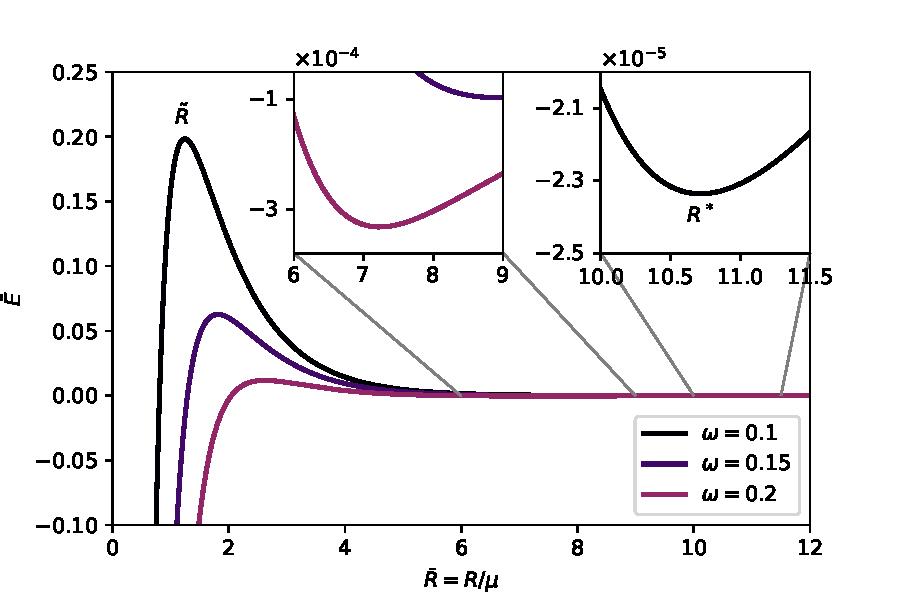
\includegraphics[width=12cm]{figures/3-elastic-figs/Epi2pi2_multiple_w.pdf}
\caption{Two body strong-strong interaction. This is the regime we focus on. The maximum $\bar{E}$ defines the $\tilde{R}$ and the stable equilibrium at $R^*$ is shown in the inset.}
\label{fig:ss}
\end{figure}
\begin{figure}[h]
\centering
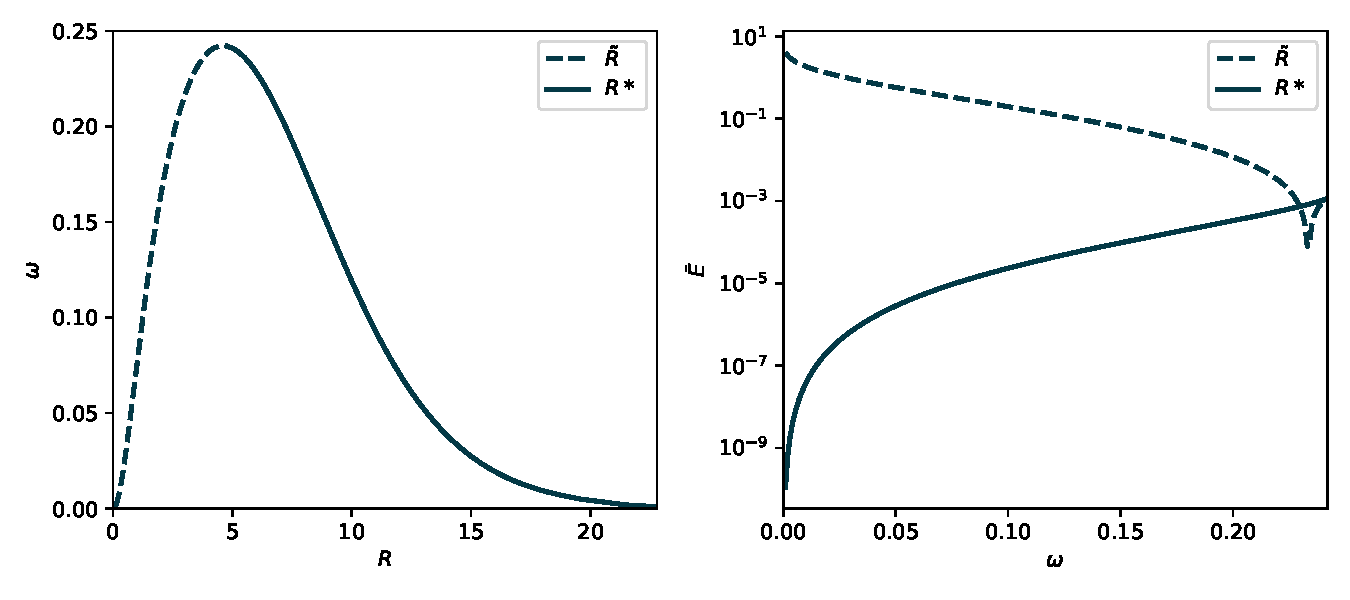
\includegraphics[width=12cm]{figures/3-elastic-figs/bifucation_di_energy.pdf}
\caption{Bifurcation diagram showing how the existence of equilibrium solutions depends the anisotropy parameter, $\omega$. The two colours are the $\tilde{R}$ and $R^*$ equilibria.}
\label{fig:Rbifur}
\end{figure}

\section{Systems of Interacting Inclusions}

Armed with this potential describing the interactions between curvature inducing inclusions, we can explore the structures and dynamics of various configurations of inclusions. The mosaic structure of the lipid bilayer allows for in plane fluid flows with high viscosity. Forces acting on inclusions embedded in a lipid bilayer will therefore cause motion as the flows allow the system to relax and find an energy minimum. Due to the high viscosity, we expect the motion to be overdamped and so each inclusion undergoes a gradient descent in the energy of the system, given by the interaction potential derived earlier. Continuing with the flat membrane approximation, we take the gradient in the $x-y$ reference plane which we used to construct the Monge parameterisation. Following equation \ref{eq:efull} we write the energy of the system as
\begin{equation}
        E= TA_0 + \kappa\xi^2 E'
\end{equation}
where $TA_0$ is constant and $E'$ is the nondimensional energy that we minimised over. The motion of each variable follows
\begin{equation}
    \dot{q_i} = \mu_q \times F_{q_i} =-\mu_q \frac{\partial E}{\partial q_i}.
\end{equation}
where $q$ is either $x$, $y$, or $\phi$. When the energy is at a minimum in all variables, the configuration will not evolve in time and we call this a stationary configuration. The evolution of the non-dimensionalised variable now becomes
\begin{equation}
    \dot{\bar{q_i}} = -\underbrace{\mu_q \frac{\mu^2}{\kappa \xi^2\alpha^2\pi L^2}}_{\bar{\mu}_q}\frac{\partial \bar{E}}{\partial \bar{q_i}}
    \label{eq:overdamp}
\end{equation}
where $\bar{\mu}_q$ has units of inverse time.  From the $x-y$ symmetry of an infinite membrane, we expect $\bar{\mu}_x = \bar{\mu}_y$ and mobilities are connected to diffusivities via the Einstein relation ($D=\mu k_B T$). The ratio of the translational and rotational diffusivity $D_T/D_R\sim a^2$ where $a$ is the radius of the circular inclusion and $a \ll 1$. As such we expect that $\bar{\mu}_x, \bar{\mu}_y \gg \bar{\mu}_{\psi}$ so that the orientation of the inclusions relaxes much faster than position. Here we often take $\bar{\mu}_{\psi} = 10 \bar{\mu}_x = 10\bar{\mu}_y$ and time is non-dimensionalised by $t \rightarrow  t'/\bar{\mu}_x$. \todo{Could we also make a scaling argument here about how these parameters should scale with $L$? This might make more sense that to use Einstein relation which raises questions about modelling the noise. \cite{chou_statistical_2001} rotational timescales usually less than translational.}

\section{Rings, Lines and Lattices}

\subsection{Rings}

There are many possible ways to arrange $n$ inclusions, with each inclusion being described by two positional coordinates an angle describing the orientation. This creates a huge space of possible inclusion configurations, however one particularly simple choice is to consider inclusions spaced evenly on a circle. We can explore the stability of such configurations and ask how this stability changes depending on the asymmetry parameter ($\omega$), or the spacing between the inclusions. We restrict the study of configurations where all inclusions are separated by at least $\Tilde{R}$ to prevent the collapse of structures caused by diverging interaction energy for small separations.

The ring is parameterised by the number of inclusions, $n$, and their distance, $l$, from a central point. This forms a regular polygon of edge length $l_e = 2l\sin(\pi/n)$ - the separation between neighbouring inclusions. We label each inclusion from $1$ to $n$ with the $i^{\text{th}}$ at position $(l\cos(2\pi i/n),l\sin(2\pi i/n))$ however, there are two choices of $\psi_i$ for the inclusions to form a maximally symmetric arrangement. These arrangements are when the the axis of each inclusion either points radially ($\psi_i = 2\pi/i$) or tangentially ($\psi_i = 2\pi/i+\pi/2$) and Fig. \ref{fig:polys2ring} shows these configurations. We can calculate the energy as a function of the radial separation. Numbering the inclusions from $1$ to $n$, the energy for a symmetric arrangement of $n$ inclusions is given by
\begin{equation}
\bar{E}_{n}(l) = \frac{n}{2}\sum_{i=1}^{n-1} \bar{E}_{xy}(l,l\cos(2\pi i/n),0,l\sin(2\pi i/n),0,2\pi i/n)
\label{eq:ring_sum}
\end{equation}
where rather than summing over all pairs we just note the $n$-fold rotational symmetry. The factor $n/2$ prevents double counting and when $n=2$, we recover the two body interaction energy, $\bar{E}_2 = \bar{E}_{xy}\left(x_1,x_2,y_1,y_2,\psi_1,\psi_2\right)$ given by (\ref{eq:exy}).

\begin{figure}[h!]
\centering
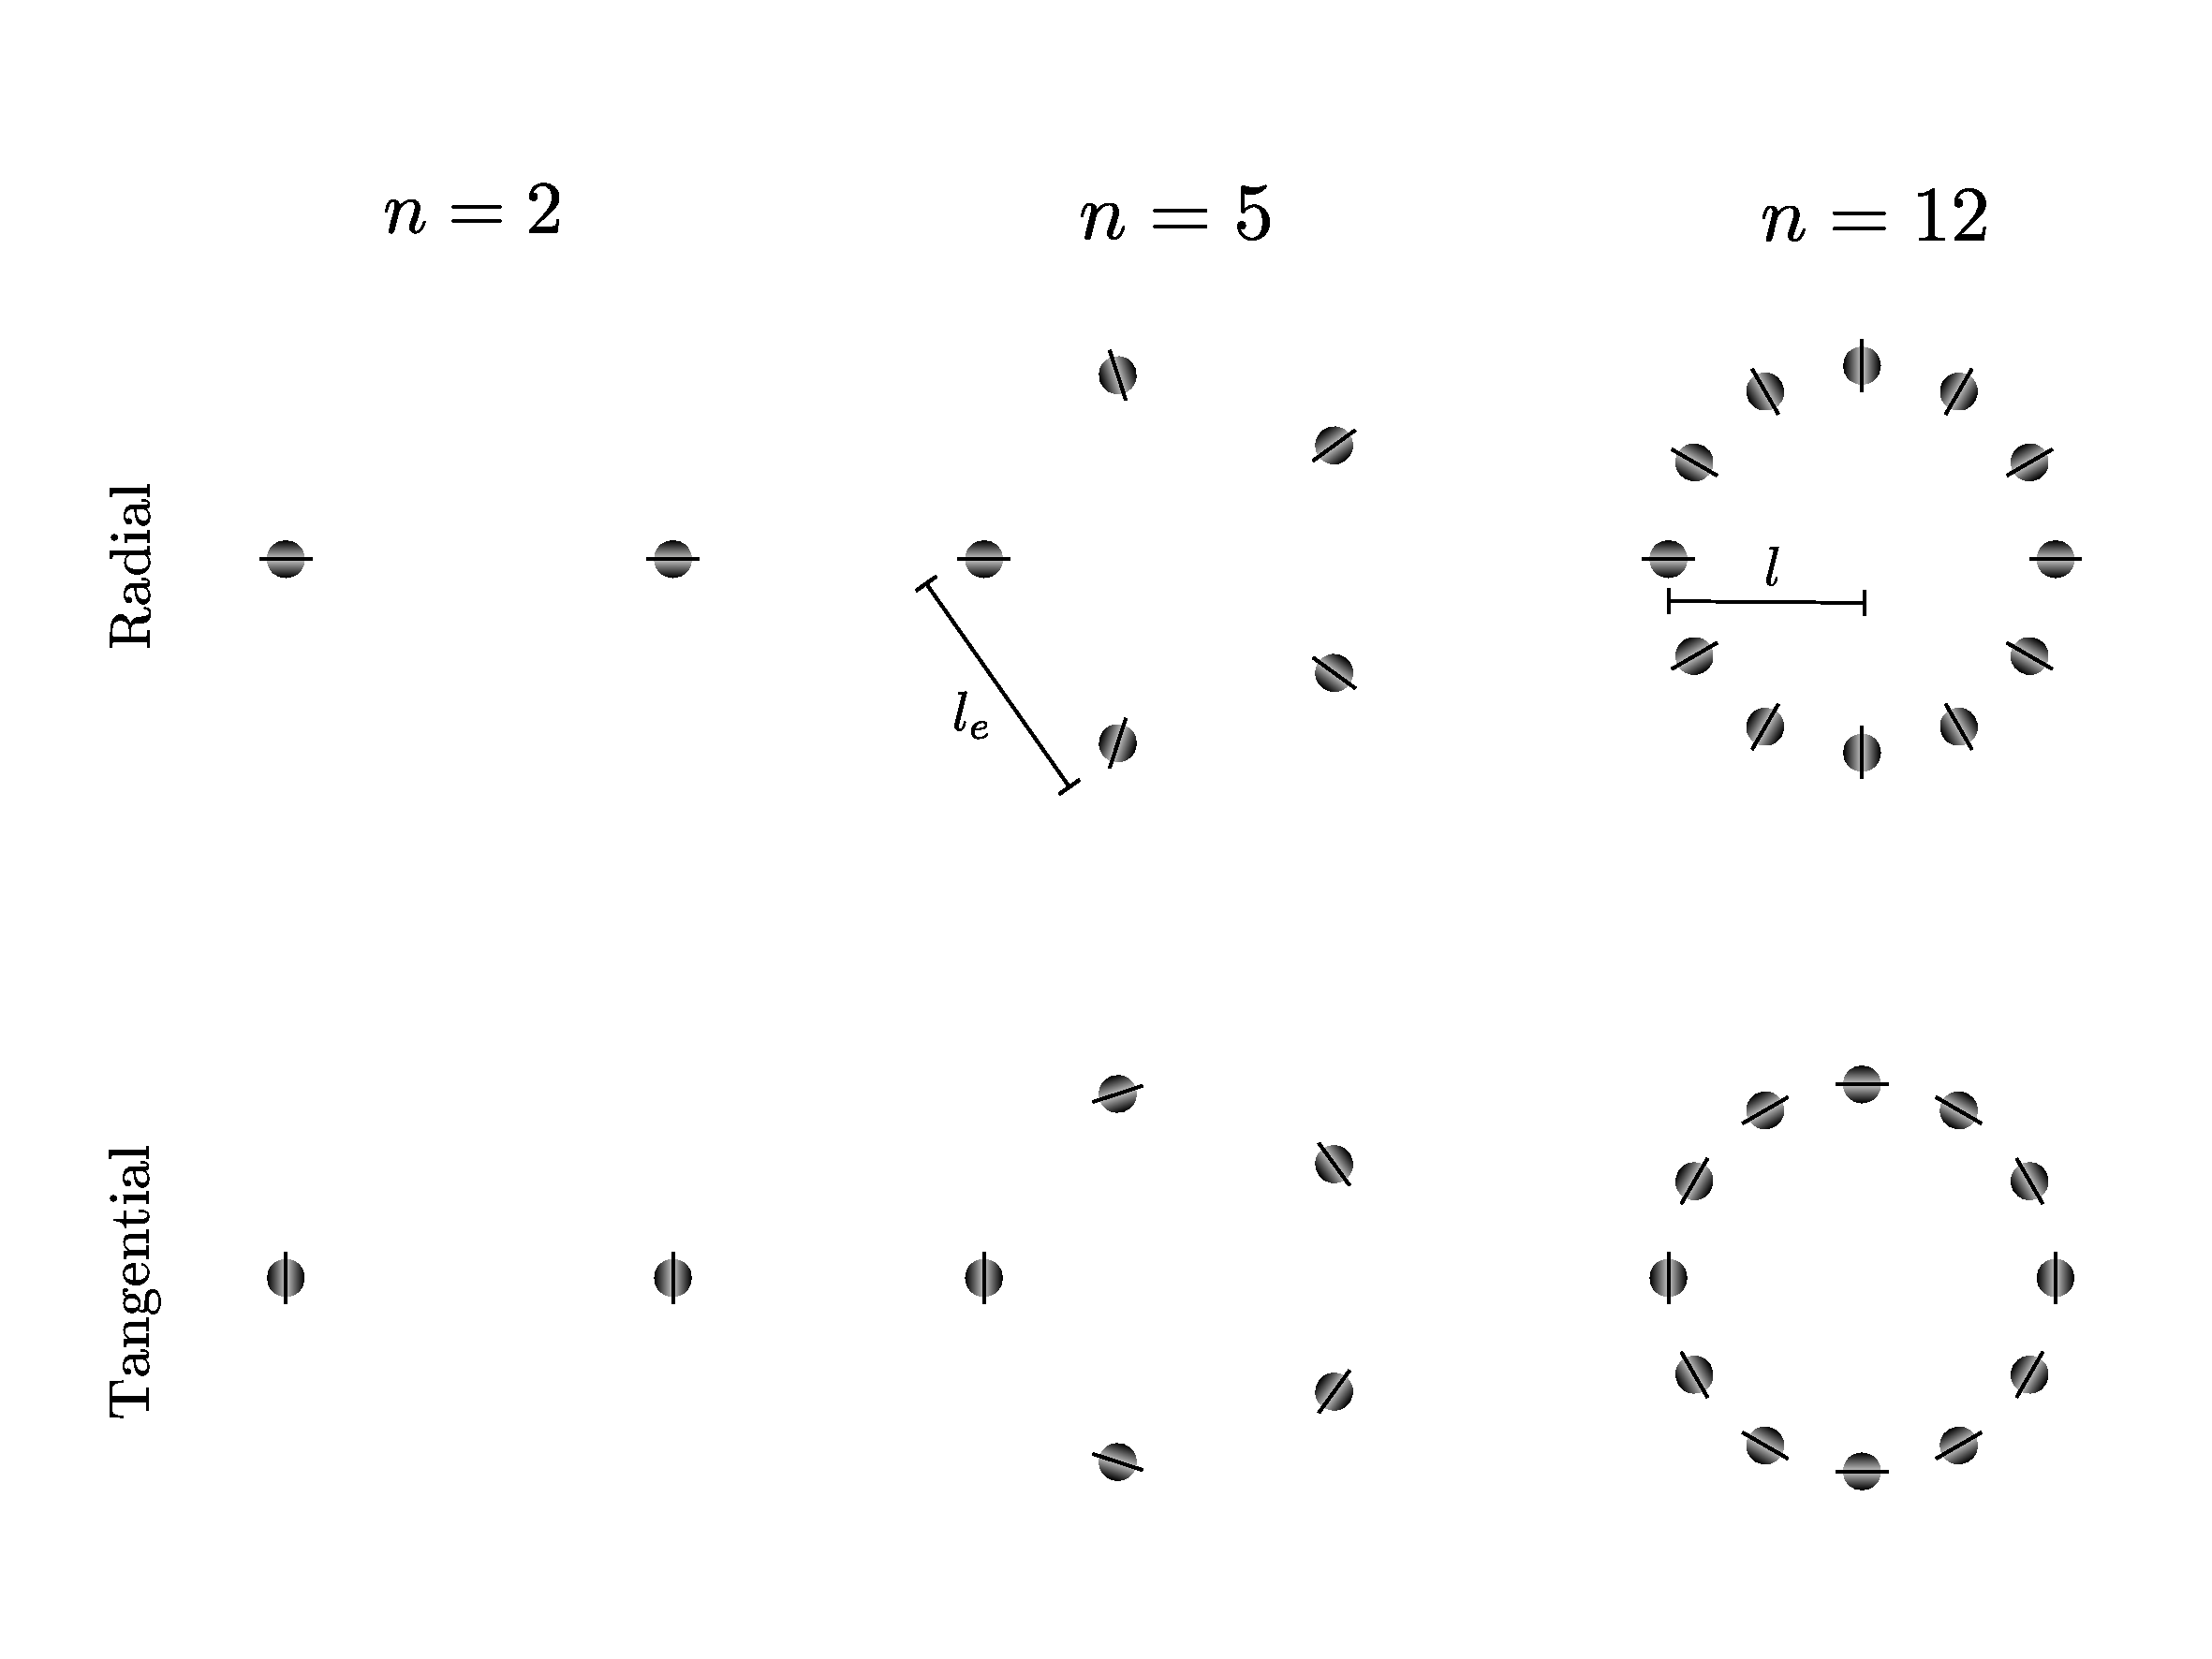
\includegraphics[width=14cm]{figures/3-elastic-figs/n_rings.pdf}
\caption{Radial and tangential setup for rings of $n=2,5,12$.}
\label{fig:polys2ring}
\end{figure}

For a ring of $n$ inclusions, there is some edge length, $l_e(n)$ that minimises the energy of the configuration. This equilibrium ring size can be determined numerically and is shown in Figure \ref{fig:Efnl} for varying $n$ and for two different values of $\omega$. There are two different values of $l_e$ for each $n$: the inclusion separation that minimises the radial configuration, $l_e^R(n)$, and similarly for the tangential configuration $l_e^T(n)$.

\begin{figure}[h]
\centering
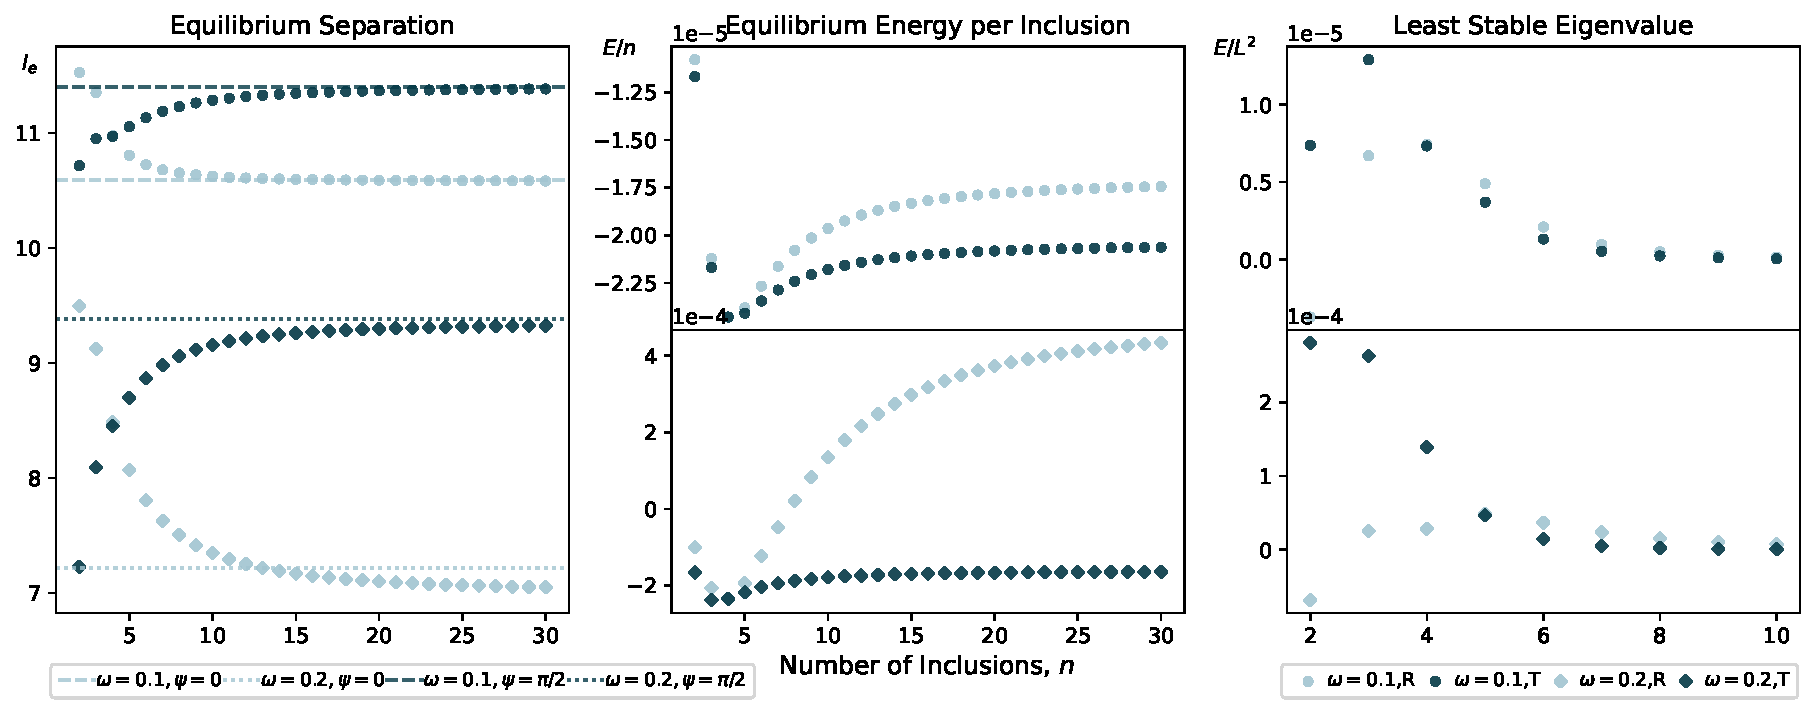
\includegraphics[width=15cm]{figures/3-elastic-figs/polys_multiple_w.pdf}
\caption{Equilibrium inclusion to inclusion separation for inclusions with $\omega=0.1$. Both the radial and tangential configurations are shown. The radial configuration all have $\psi^R_i=2\pi i/n$, compared to the tangential case of $\psi^T_i=2\pi i/n+\pi/2$. \todo{Haven't been able to figure out the $\omega=0.2, \psi=0$ doesn't line up.}}
\label{fig:Efnl}
\end{figure}

As $n$ becomes larger $l_e^T(n)$ is closer to $l_e^R(2)$ than $l_e^T(2)$ (and similarly the other way around). This can be understood as follows: for large $n$, adjacent inclusions in the tangential configuration look very similar to the radial configuration of the two inclusion case i.e. nearest neighbours for $n=12$ in Fig. \ref{fig:polys2ring} look similar to the setup in the $n=2$ case on the left of the figure. The graph also shows that $l_e^T(4) \approx l_e^R(4)$. This makes sense since the symmetry of the two body interaction means that the adjacent inclusions have the same interaction energy in both the radial and tangential configurations and the only difference between the two configurations is come from the pairs of diagonal inclusions. In fact, only the diagonal energy term that is proportional to $(\cos2\psi_1+\cos2\psi_2)$ is different, between the two arrangements.

The stability of a configuration of inclusions can be determined by studying the eigenvalues of the energy Hessian matrix, $\mathbf{H}$ evaluated at the configuration. Here, the Hessian is defined as
\begin{equation}
    \mathbf{H}_{ij}=\frac{\partial^2 \bar{E}}{\partial q_i \partial q_j}.
\end{equation}
If the Hessian is positive semidefinite, $\mathbf{H} \succeq 0$, all of the eigenvalues are positive and the energy increases under any perturbation. This means the equilibrium is stable and under the overdamped dynamics, the system will approach this minimum state from other configurations in the basin attraction. The Hessian and the eigenvalues can be calculated for finite rings and for ring sizes. For any $n$ there are three zero eigenvalues that correspond to the symmetries of the energy: two orthogonal translations of all inclusions and a rotation of the position and angle of all inclusions. In addition to these modes, for $n>2$ all other perturbations increased the energy of the system and rings of inclusions of all sizes are stable.

The Hessian, $\mathbf{H}$, is a $3n\times3n$ matrix and for larger numbers of inclusions, it is hard to extract any meaning from the resulting eigenvectors. Since we expect the translational dynamics to be much slower than the rotational dynamics, we can reduce the number of degrees of freedom by considering only the rotational degree of freedom for each inclusion. Perturbations in the angle are always stable, however it is instructive to study the corresponding eigenmodes. When $n$ is even for both the radial and tangential configurations, the least stable mode - i.e. the mode with the least positive eigenvalue - is a mode with the angles all perturbed by the same magnitude, but with alternating sign between adjacent inclusions, i.e. $\delta\phi_i = (-1)^{i}|\delta\phi|$. For rings with odd numbers of inclusions these alternating rotations would create a mismatch between the first and $n^{\text{th}}$ inclusions and so this might not be the least stable mode. In fact, when $n$ is odd and not very small, the eigenvector with the lowest eigenvalue still corresponded to rotating adjacent inclusions in opposite directions however the magnitude of these rotations varies in such a way that at the mismatch the magnitude of the rotation is very small. When $n=2$, the equivalent radial configuration is unstable, however and the unstable mode is given by an equal and opposite rotation of each inclusion.
% \todo{maybe link to the 2 body interaction}

% \begin{figure}[h]
% \centering
% 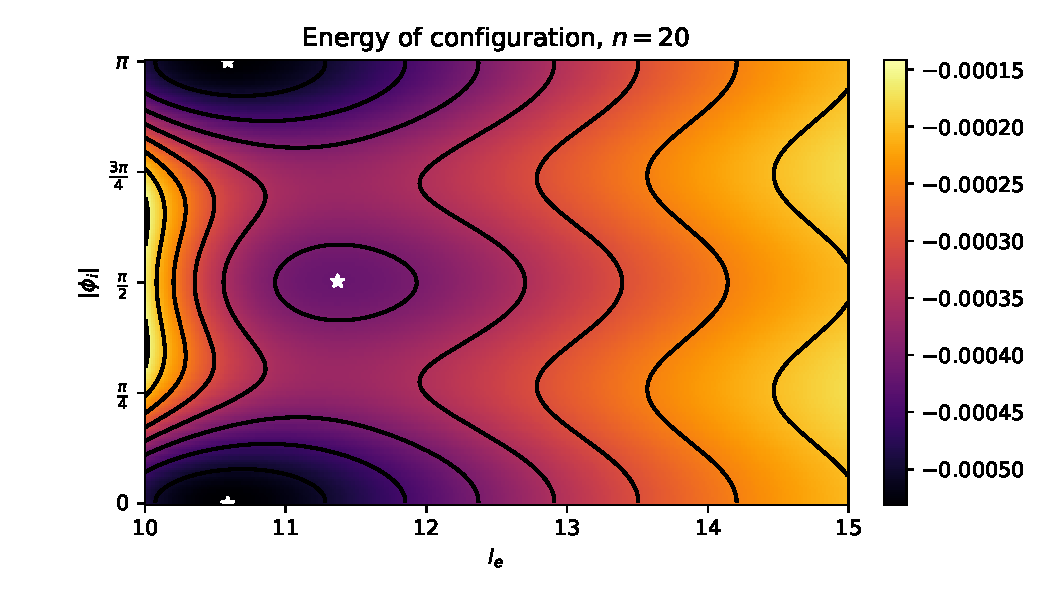
\includegraphics[width=12cm]{figures/3-elastic-figs/ring20sized2.pdf}
% \caption{Interaction energy for a ring of $n=20$ inclusions. The energy is plotted as the inclusion separation and alternating mode perturbation are varied.}
% \label{fig:ring20}
% \end{figure}
\notyet{
\begin{figure}[h!]
\centering
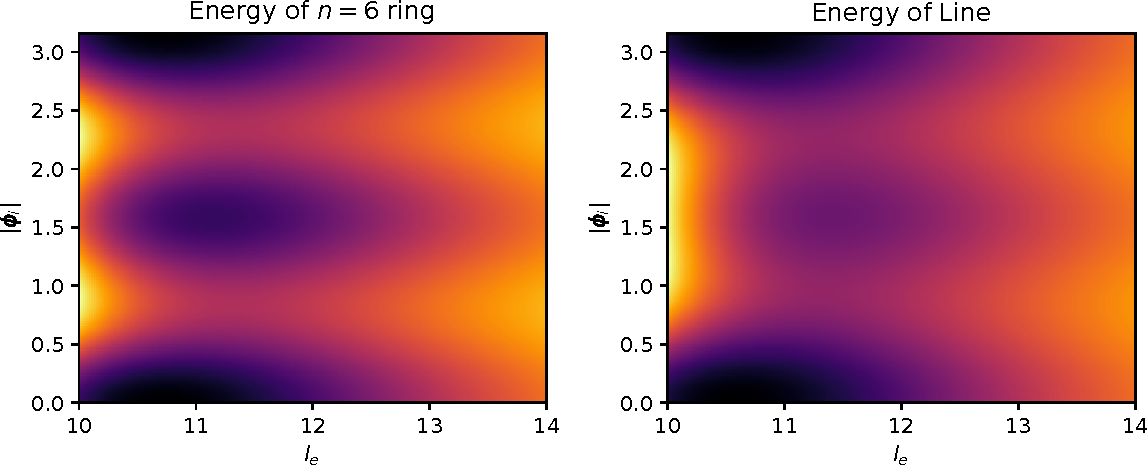
\includegraphics[width=15cm]{figures/3-elastic-figs/energy_line_vs_6_tight.pdf}
\caption{Interaction energy per inclusion for an infinite line inclusions and for a ring of $n=6$ inclusions. The energy is plotted as the inclusion separation and alternating mode perturbation are varied.}
\label{fig:lineenergy}
\end{figure}
}
\begin{figure}[h!]
\centering
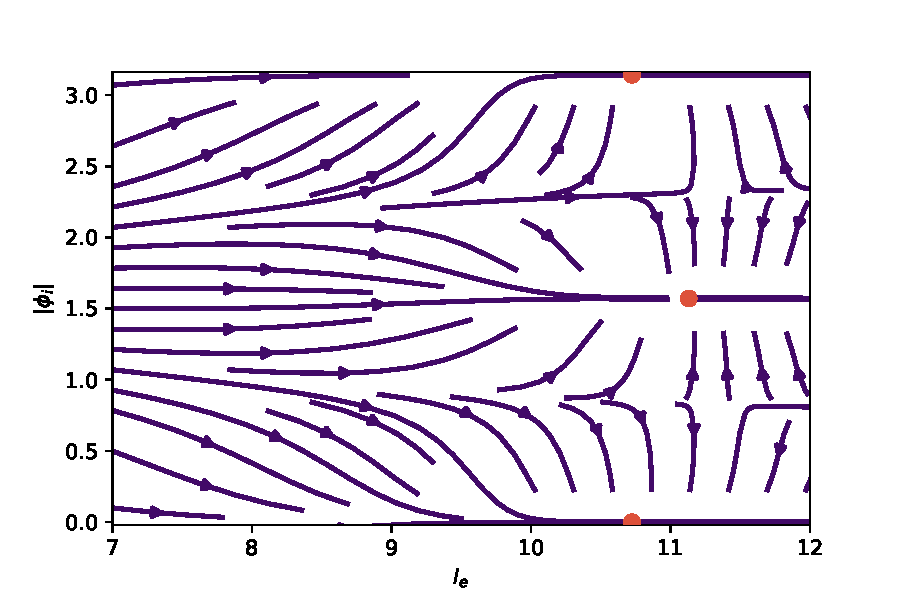
\includegraphics[width=12cm]{figures/3-elastic-figs/streams.pdf}
\caption{Stream plot showing gradient descent for a ring of inclusions in the reduced paramter space of the alternating angular modes at various inclusion-to-inclusion separations. Shown for n=[], $\omega=0.1$ and the key featrures are the same for $\omega=0.2$.}
\label{fig:ring_stream}
\end{figure}

Focusing on a ring with even $n$ number of inclusions, this vector with alternating signs for the rotation connects the radial and tangential configurations. For example starting at the radial configuration, if we perturb all angles by $\delta\phi_i = (-1)^{i}\pi/2$, the system will transition to the tangential configuration. This path represents a trajectory between the two configurations with constant ring radius $l_e$ that initially requires the minimum energy. Varying this parameter, $|\delta\phi|$, and $l_e$ we can explore the energy landscape of these configurations in a massively reduced parameter space that will still give a good representation of the stability of the system. \notyet{\todo{can we get an energy barrier in this space for these?}}

Fig. \ref{fig:ring_stream} shows the gradient descent flow of a ring of inclusions constrained to be evenly radially distributed with an inter inclusion length of $l_e$, and with orientation perturbations that alternate when measured from the radial configuration. The minima for the two maximally symmetric cases are shown by the red dots and as expected the system will approach these two stable configurations anywhere in the phase space. At large $l_e$ the system will approach the nearest configuration in angular space, however at low separations the system approaches the radial ($|\phi_i|=0$) configuration for a wider range of angles. Despite being a subspace of all possible configurations, this observation is informative of the basin of attraction of these two equilibria in all configuration space and indeed when simulating the gradient descent of a random set of pertubations, it is observed that the radial emerges when systems are initialised at smaller $l_e$.

% \subsubsection{Potential from Rings}
% Rings of inclusions will still interact with other inclusions in the pairwise fashion. An additional inclusion outside of a ring of inclusions will cause a minor perturbation of the equilibrium separation of the ring and so we model the ring as being fixed at it's unperturbed separation. If we ignore this minor perturbation, the interaction potential felt by an external inclusion is the sum of contributions from each inclusion in the ring. This interaction is described by three parameters: the  separation between the inclusion and the centre of the ring  $R_\text{ext}$, the angle of the  inclusion $\psi_i$, and the global rotation of the ring $\psi_r$. \todo{Dont even think that the equation below is correct!? - brackets issues I think}
% \begin{equation}
%     E_{\text{ext}} = \sum_N E_2(\sqrt{R_\text{ext}+l_e\sin(2\pi N/5 + \psi_r)^2+l_e\cos(2\pi N/5 + \psi_r)^2}, 2\pi N/5), 
% \end{equation}
% \begin{figure}[h]
% \centering
% \includegraphics[width=12cm]{figures/3-elastic-figs/ring20lower.pdf}
% \caption{Interaction energy for a ring of $n=20$ inclusions at closer separations. The energy is plotted as the inclusion separation and alternating mode perturbation are varied.}
% \label{fig:ring20lower}
% \end{figure}

% \subsection{Random Thoughts}

% Compare e.g. a lattice of size with a ring with all inclusions in there

% Here we investigate the lower density structure formed by anisotropic inclusions and focus on the sturtures that form in the limit of lower densities.

% In this dilute limit, L is large and therefore tension is strong..?

\subsection{Lines}

\subsubsection{Infinite Lines}
As the number of inclusions in the ring increases, the length between neighbouring inclusions, $l_e$, converges to a constant equilibrium value and the ring radius tends to infinity. In the limit this ring of inclusions becomes a line of inclusions separated by $l_e$, and with all inclusions having the same orientation, either $\psi_i=0$ or $\pi/2$ which are analogous to the limits of the tangential or radial rings respectively. Similarly to rings of inclusions, we can explore the energy landscape of the line. Since there are infinitely many inclusions, we expect the energy of the configuration to be infinite. The energy of the interacting inclusions will still be pairwise and as such
\begin{align}
    \bar{E}_{line} &= \sum_{i\neq j}\bar{E}_2(R_{ij}, \pi/2, \pi/2) = \sum_{i=-\infty}^{\infty}\sum_{j=i+1}^{\infty}\bar{E}_2(R_{ij}, \pi/2, \pi/2) \\
    &= \frac{1}{2}\sum_{i=-\infty}^{\infty}\sum_{j=1}^{\infty}\left(\bar{E}_2(l_e \times j, \pi/2, \pi/2) + \bar{E}_2(-l_e \times j, \pi/2, \pi/2)\right) \\
    &= \sum_{i=-\infty}^{\infty}\sum_{j=1}^{\infty}\bar{E}_2(l_e \times j, \pi/2, \pi/2) 
\end{align}
where we can identify the energy \textit{per inclusion} of the line as $\sum_{j=1}^{\infty}\bar{E}_2(l_e \times j, \pi/2, \pi/2)$. \notyet{Approximating the sums as integrals using the Euler-Maclaurin formula gives a very large error. However, we expect that this sum will converge due to the form of the pairwise interaction.}When $x$ is large, $K_\nu(x)\sim e^{-x}/\sqrt{x}$ and therefore $\sum_{n=1}^\infty K_\nu(nx)$ will converge. We also have $\sum_{n=1}^\infty(1/n^4) = \pi^4/90$ and so the energy per inclusion in an infinite line will be finite.\todo{does this make sense? do we need to talk about the density instead?} The sum over all inclusions can be evaluated and is shown in \todo{Fig \ref{}}.
\notyet{The Bessel functions in the two-inclusion interaction energy decay exponentially with distance in the far field and so the sum of $\sum_i K_0(l_e \times i)$ will converge, as will the sums for the other Bessel functions. The remaining term in the energy $\sim\sum_i R^{(l_e \times i)}$ also converges and can be calculated directly.}
% (https://math.stackexchange.com/questions/650966/evaluate-sum-infty-n-1-frac1n4-using-parsevals-theorem-fourier-ser).
% The Euler–Maclaurin formula can convert sums to integrals upto some correction term. This can convert the sum of infinite Bessel function into an integral, however this provides bad accuracy. For example, consider the term in the energy that goes like $K_{0}(R)$. This term's contribution to the energy per inclusion is given by 
% \begin{equation}
%     \sum_{i=1}^{\infty}E_2(i\times l, \phi_i) =
%     \int_m^{n}f(x)dx + \sum _{k=1}^{p}{{\frac {B_{k}}{k!}}\left(f^{(k-1)}(n)-f^{(k-1)}(m)\right)}+R_{p}
% \end{equation}
% \begin{align}
%     \sum_{i=1}^{\infty}E_2(i\times l, \phi_i) &=
%     \int_m^{n}f(x)dx + \sum _{k=1}^{p}{{\frac {B_{k}}{k!}}\left(f^{(k-1)}(n)-f^{(k-1)}(m)\right)}+R_{p} \\
%     &={\frac {f(m)+f(n)}{2}}+{\frac {1}{6}}{\frac {f'(n)-f'(m)}{2!}}-{\frac {1}{30}}{\frac {f'''(n)-f'''(m)}{4!}}+{\frac {1}{42}}{\frac {f^{(5)}(n)-f^{(5)}(m)}{6!}}-\int _{m}^{n}f^{(6)}(x){\frac {P_{6}(x)}{6!}}\,dx\\
% \end{align}
% #####
For rings of inclusions, often we studied the least stable perturbation of the orientations of the inclusions, where each inclusion is rotated by the amount but in opposite directions. A line of inclusions can be perturbed in the same way and again this will transition between a configuration with $\psi_i=0$ to $\psi_i=\pi/2$ for all inclusions, $i$. The energy of a system with $\psi_i=\pm|\delta\phi|$ is given by summing over the inclusions that are rotated in the opposite and same direction separately. The energy of the perturbed line is given by  
\begin{equation}
    E^*_{alt}(\delta\phi) = \sum_{j=1,\text{ odd}}^{\infty}\bar{E}_2(l_e \times j, \pi/2+\delta\phi, \pi/2-\delta\phi) + \sum_{j=2,\text{  even}}^{\infty}\bar{E}_2(l_e \times j, \pi/2+\delta\phi, \pi/2+\delta\phi)
\end{equation}
which simplifies to
\begin{equation}
    \begin{split}
    E^*_{alt}(\delta\phi) =&2\sum_{all}K_0(l_e \times i) - 4\omega\cos(2\delta\phi)\sum_{all}K_2(l_e \times i)+ \omega^2\sum_{even}K_0(l_e \times i)\\
    &+ \omega^2\cos(4\delta\phi)\sum_{odd}K_0(l_e \times i) + \omega^2\cos(4\delta\phi)\sum_{even}\left(K_4(l_e \times i)-\frac{48}{(l_e \times i)^4}\right)
    \end{split}
\end{equation}
and which we can plot, analogously to Fig. \ref{fig:ring20}. The energy profile for the line is shown in Fig. \ref{fig:lineenergy}.
% \begin{figure}[h]
% \centering
% 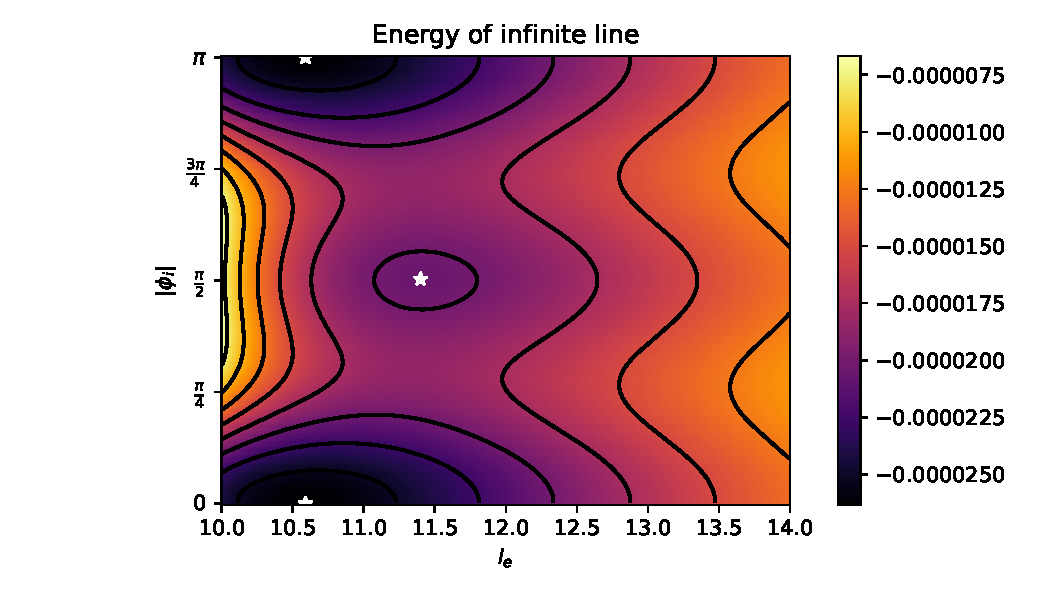
\includegraphics[width=12cm]{figures/3-elastic-figs/line_anti.pdf}
% \caption{Interaction energy per inclusion for an infinite line inclusions. The energy is plotted as the inclusion separation and alternating mode perturbation are varied.}
% \label{fig:lineenergy}
% \end{figure}
Similarly to the rings, the line is stable for both $\psi_i=0$ and $\psi_i=\pi/2$ (for all $i$). The energy minimum is much deeper when $\psi_i=\pi/2$ and this configuration is likely to also have a larger basin of attraction than when $\psi_i=0$. This configuration corresponds to an end-to-end alignment of inclusions with anisotropic geometry\cite{kwiecinski_interactions_2020} and linear aggregates with similar structure have been observed experimentally\cite{simunovic_long-range_2017} and in molecular dynamics simulations \cite{simunovic_linear_2013}. The structure then localises to membrane buds and shows the relevance of elastic interactions even at low densities.

\todo{Is there a way to calculate the energy eigenvalues around stable line?}
\todo{The infinite line stabilises the unstable 2-body interaction.}

\subsubsection{Finite Lines}
Lines with a finite number of inclusions are relevant to study for physically realisable finite systems. The existence of a infinite line would require an infinite system, but also it's likely that shorter lines made up of fewer inclusions will form as intermediates if longer (or even infinite) lines of inclusions were to form. Again, there are two obvious orientations of inclusions to study, but unlike the infinite line each inclusion sees a different arrangement of the other inclusions. As such the equilibrium separation between neighbouring inclusions is not constant but its perturbed slightly depending on their position along the line. The more central inclusions on the lines have a slightly lower separation that those closer to the ends, however this variation was seen to be at most a change of around $2\%$ in the separation across the different inclusions, with the inclusions on the end of the line being more separated.

Again, by studying the Hessian of energy at this stationary configuration, we observe that a finite line of inclusions along the x-axis with the inclusions orientated at $\psi_i=\pi/2$ is stable. This is the configuration similar to the radial ring configuration. However, when the inclusions are orientated at $\psi_i=0$, the finite line is no longer unstable (the tangential ring). For the specific case of a finite line of two inclusions, we saw earlier only one angular orientation was stable. Larger, but still finite lines of inclusions remain unstable and in particular a long oscillatory mode is excited as the line transitions into another configuration. \notyet{\todo{... Talk about the unstable mode}} However, the tangential ring stabilises the two body interaction as exciting the unstable mode would lead to frustration in the system and subsequently raise the energy of the configuration.


\todo{Maybe wait until talking about general configurations/evolution.} Two or more stable finite lines will interact via the elastic mediated interaction. Allowing a group of finite lines to evolve subject to this potential we find that short lines, such as pairs or three co-linear inclusions, will rotate so that their orientations align and then attract to form a large finite line. For larger co-linear groups of inclusions, the initial distribution of the lines can affect the final configuration. As an example, a group of inclusions that approach a line perpendicular to the line of the inclusions will generate different interactions with the different inclusions in the line. As the groups of inclusions approach, this difference in interaction can become large enough to bend the line and transition into a radial ring of inclusions. If the two finite lines of inclusion are aligned initially (but with a spacing to form distinct groups), then the lines will simply coalesce into a longer line. As such, the final configuration depends on the initial distributions of the lines.

\subsection{General Configurations}
Studying rings and lines is useful as these configurations massively reduce the number of coordinates needed to describe the system. However observed inclusion configurations can be initially generated by diffusing proteins binding onto the membranes or as a consequence of driven cellular process that may drag inclusions before detaching. It is therefore useful to explore the elastic forces acting on generic inclusion arrangements which will not necessarily be as symmetric as the rings and lines.

We can explore the evolution of a generic configuration by evolving the system to respond to gradients in energy in the overdamped regime, following the dynamics in (\ref{eq:overdamp}). We choose $\Bar{\mu}_x=\Bar{\mu}_y=\mu_{\phi}/10$, so that the inclusions rotate more quickly in response to gradients of a free energy than they translate and the system is initialised in a random starting configuration with all separations between inclusions greater than $\tilde{R}$. Ensuring this initial separation prevents any of the inclusions from collapsing with diverging energy and allows us to observe the subsequent relaxation of the system to a minimum energy configuration.

As the system is allowed to evolve according to the gradient descent dynamics, the inclusions begin to form aggregates. The system relaxes to a low energy state, where each inclusion is surrounded by a set of neighbouring inclusions that are all approximately $R^*$ away. This makes sense, the interaction from nearby inclusions gives the main contribution to the interaction energy and so the system will try to minimise the two body interaction energy for neighbouring inclusions, however this equilibrium will be slightly perturbed by inclusions that are further away. Similarly to rings, the non-neighbouring inclusions will perturb both the separation and orientation away from being exactly at the two-body equilibrium, and in particular, the anisotropy of the inclusions can generate frustration alter the orientation that minimises the energy.

To visualise the structure of the aggregates, we construct a graph and associated 2D embedding for each configuration. Each inclusion is represented by a node in the graph, embedded at the inclusion location, and edges of the graph connect nearest neighbour inclusions, which we define to be inclusions closer than a distance of $1.3R^{*}$ apart. \notyet{\todo{verify the pre-factor and be consistent}} This threshold is chosen to capture the range of nearest neighbour interactions that were seen from the stable ring and line configurations, without capturing inclusions further away. In particularly, it is good for the threshold to be less than $\sqrt{2}R^{*}$ else diagonal inclusions in a square configuration may appear as nearest neighbours. Constructing this graph and visualising the edges, many of the aggregates formed were comprised of rings of aggregates that formed a lattice of polygons. Additionally, there were also stable configurations containing lines of inclusions that protruded out from the aggregate. \todo{Samples are shown in Fig.}

\todo{some general comments about there being lots of different minimia that the system can end up in, etc., etc.}

\begin{figure}[h]
\centering
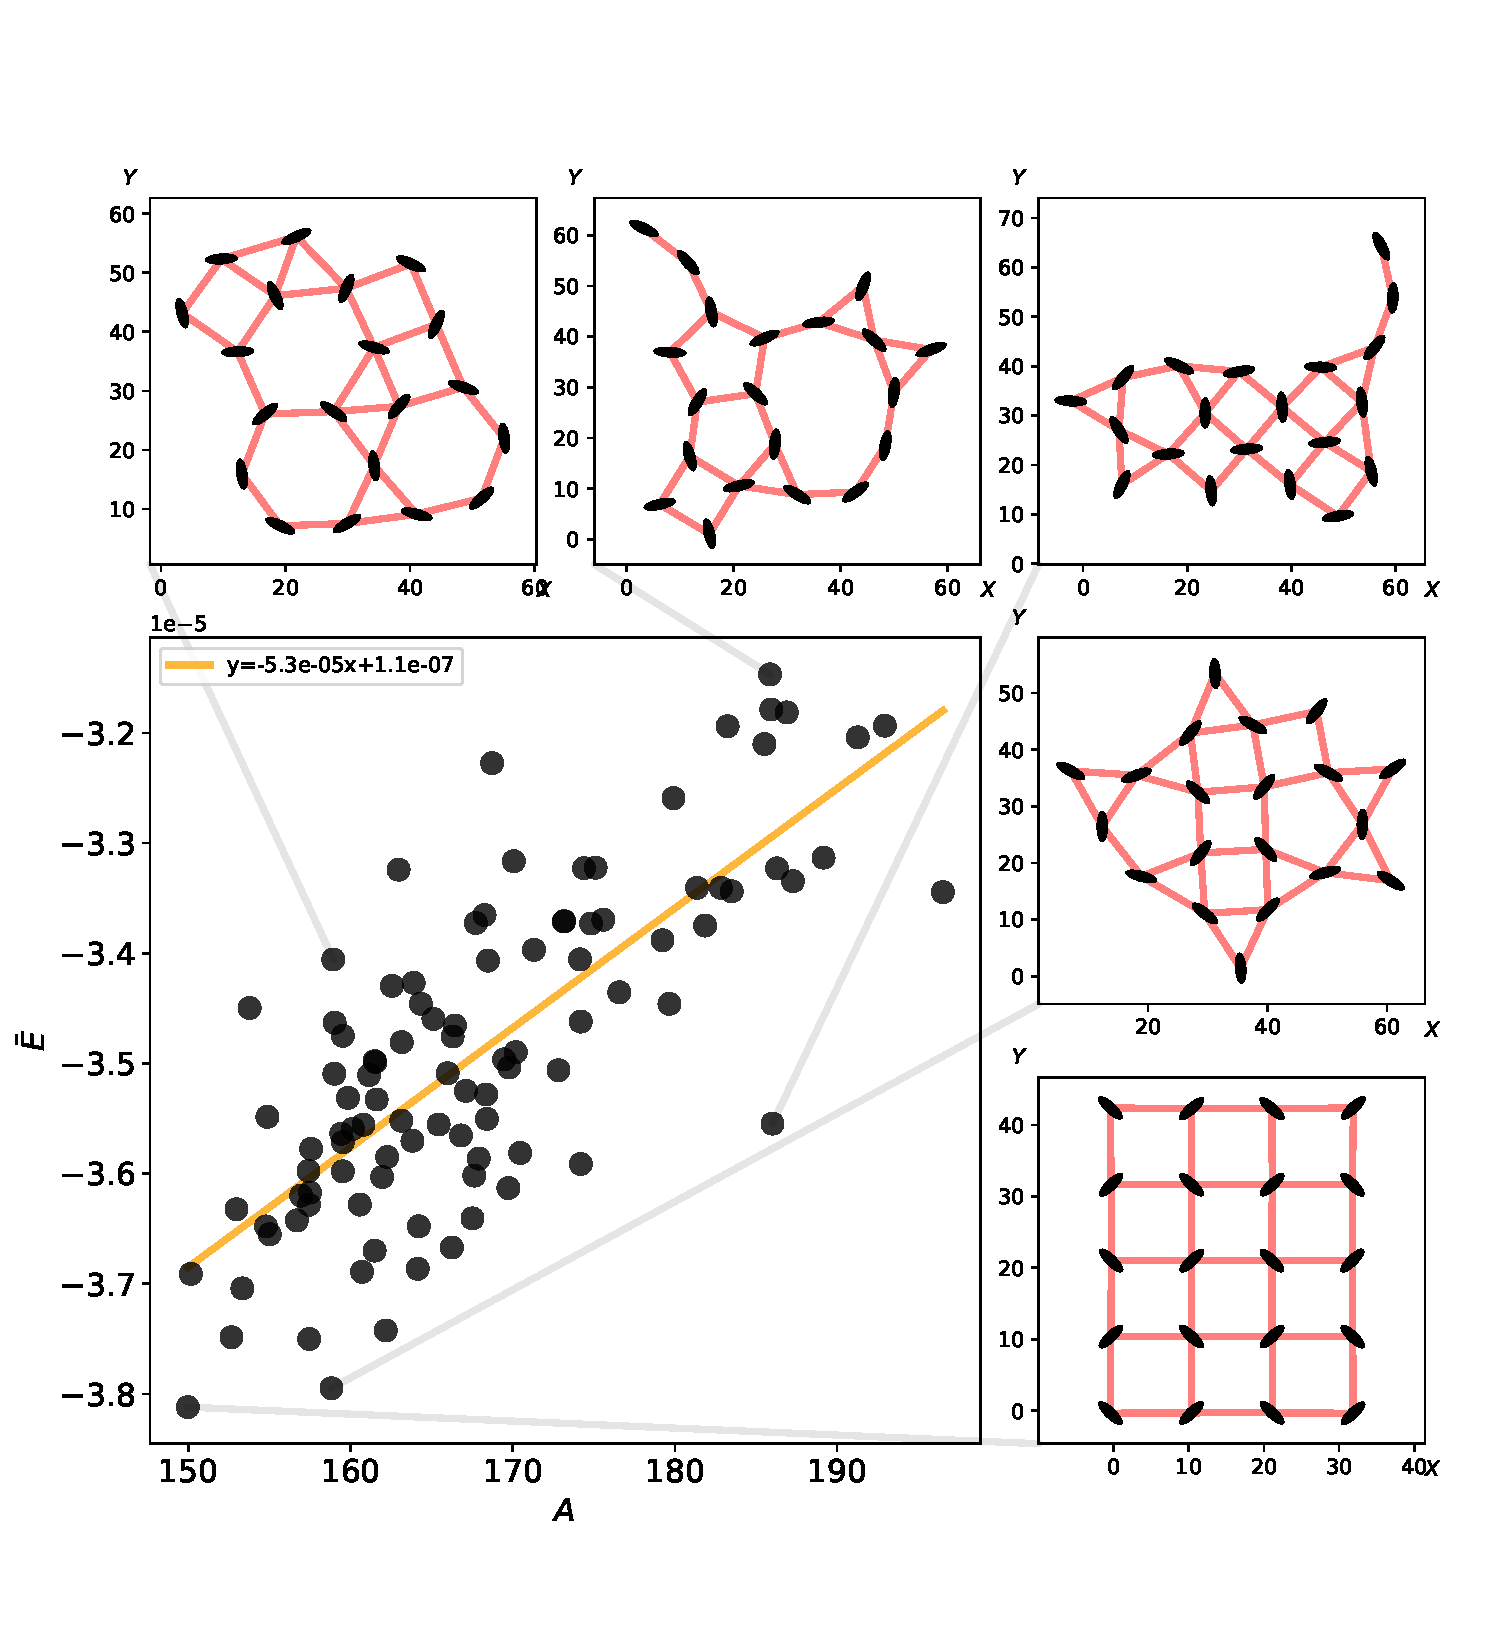
\includegraphics[width=12cm]{figures/3-elastic-figs/autoLatticeEgs100slope.pdf}
\caption{Sample Lattice Figs}
\end{figure}

\subsubsection{Aggregate Structure Depends on Initial Distribution}

The final stable configuration of inclusions depends on the initial configuration. For example, for the case of interacting finite lines the resulting inclusion configuration can be a larger line or a ring, depending on how the initial lines are orientated. This idea holds more generally, and we see a strong dependence of the final stable configuration of inclusions on the initial inclusion configuration. A starting configuration that is closely packed together (still with the minimum separation between inclusions greater than $\tilde{R}$) will initially feel a strong repulsion from nearby inclusions and the inclusions will spread out. During this process, the repulsion dominates, and transient triangular lattices with a lattice spacing less than $R^*$ emerge. As the inclusions are forced to separate by this potential, the average inter inclusion separation approaches $R^*$ and the inclusions rotate to minimise the interaction energy, forming a lattice with many rings of size four, the square configuration seen earlier. In fact, from specific starting configurations a square lattice can form, consisting exclusively of connected groups of four inclusions with alternating, chequerboard pattern of tangential and radial configurations.

In systems of many interacting inclusions, we expect that the square lattice will minimise the configuration energy. Each nearest neighbour will lower the interaction energy, since the two body contribution is negative. The square lattice is the 2D polygonal structure that maximises the number of compatible nearest neighbours and therefore minimises the energy. Not all combinations of regular polygons tile the plane and if they do, there is an additional geometric constraint on the orientation with adjacent polygons. For example, in a triangular lattice, there are six nearest neighbours, however any arrangement of inclusions will be unstable in some mode. This also means that the most dense lattice that can form is the square lattice and so when starting from a high density configuration, the system will encounter this minimum first during its relaxation to an equilibrium.

Fig. \ref{fig:latemerg} demonstrates the formation of the lattice from a random initial inclusions configuration.

\begin{figure}[h]
\centering
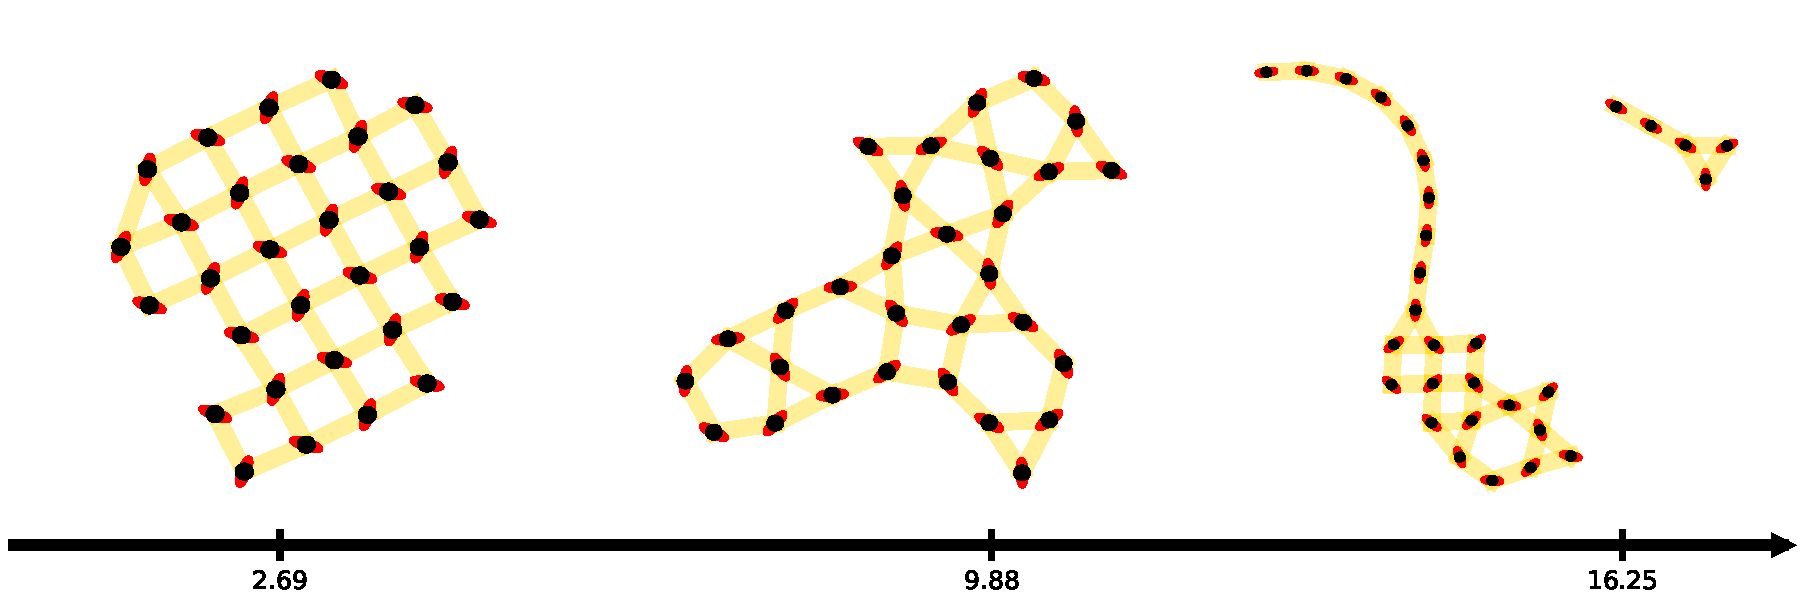
\includegraphics[width=15cm]{figures/3-elastic-figs/different_starts_sample.pdf}
\caption{Examples of the different lattice structures formed from different initial mean nearest neighbours configurations. }
\end{figure}

When inclusions are initialised further apart, all inclusions are initially attracted towards each other. The inclusions are attracted to closer inclusions more strongly and as such two inclusions will suddenly coalesce into the 2-body equilibrium configuration before coalescing with further single inclusions or group of previously coalesced inclusions. This process repeats to form aggregated structures, where groups of coalesced inclusions sequentially grow. In the very low density limit, the spacing between inclusions is very large, so that as they approach the inclusions align and are appended onto the end of existing lines. Multiple inclusions coalescing at similar times, or large lines of inclusions \todo{or just the correct angle really} can perturb the finite lines and generate rings of inclusions. Lines of inclusions will have grown before this happens and thus the rings formed are can be much larger than the polygons of size less than five typically seen for high density initial conditions.

Observed rings of inclusions formed from random configurations result in the radial equilibrium. Again, when the inclusions are initialised at large separation, they will sequentially form a chain in the equivalent of a radial configuration. If the inclusions are perturbed by other inclusions in the system, then this line will collapse into radial ring. Alternatively if multiple inclusions are intialised close together then the streamplot in Figure \todo{ref the stream plot} show that the basin of attraction for the radial configuration is larger than the tangential configuration and as such any rings formed will for a radial ring.

\subsection{Barriers between Configurations}
\todo{incoming}
\notyet{
An interesting question is to do with the transition between the different inclusions configurations. Again, due to the many complex local minima in the space of inclusion configurations, there isn't an obvious way to exhaustively explore the energy landscape and minimum energy barriers associated with transitions between the configurations. Instead, considering simple heurestics and Monte Carlo simulations we can build an intuition for this landscape and how the barriers might affect elastic interactions.

We refer to the barrier of a transition as the minimum increase in the energy required to get from one configuration to another. The transition barrier is the minimum of the maximum energy along the path between two configurations. For any two configurations there exists a path with a maximum energy of intermediate configurations that has 0 energy, which is achieved by sequentially taking the outer most inclusion to infinity and then bringing the inclusions back in one-by-one to build the target configuration. However, often the barrier will be lower than this upper limit.

A particularly simple transition between two energy configurations is the transition where an inclusion is \textit{popped} out of a structure so that a row of three inclusions becomes a triangle. For example, a ring of size $n$ transitioning to a ring of size $n-1$ with a triangular configuration attached as shown in Figure \ref{fig:popout}. 

In order to find the true barrier height, 
To find the barrier height, we would like to find a path between two configurations and minimise the maximum energy along that path. As mentioend exploreing the entire configuration space is not feasible and so instead we use the gradient descent dynamics to aid this search. For example, one might pertub an initial configuration along the direction of a low energy increase and then allow the system to evolve. If the initial perturbation was large enough then the system may approach another energy minimum. However, this approach is limited since the target configuration cannot be controlled and so an alternative approach is to smoothly vary the positional coordinates to approach the target configuration and determine the inclusion orientations by finding the minimum energy subject to inclusion rotations. Again this means that the target orientations cannot be entirely determined, but this provides a feasible method to bound the barrier height between separate configurations.

Also tried other schemes, but they dont really work , lots of time due to the symmetry in everything.   

\todo{Actually we could just start with a configuration, perturb it and allow the system to gradient descent etc.}
    
\begin{figure}[h]
\centering
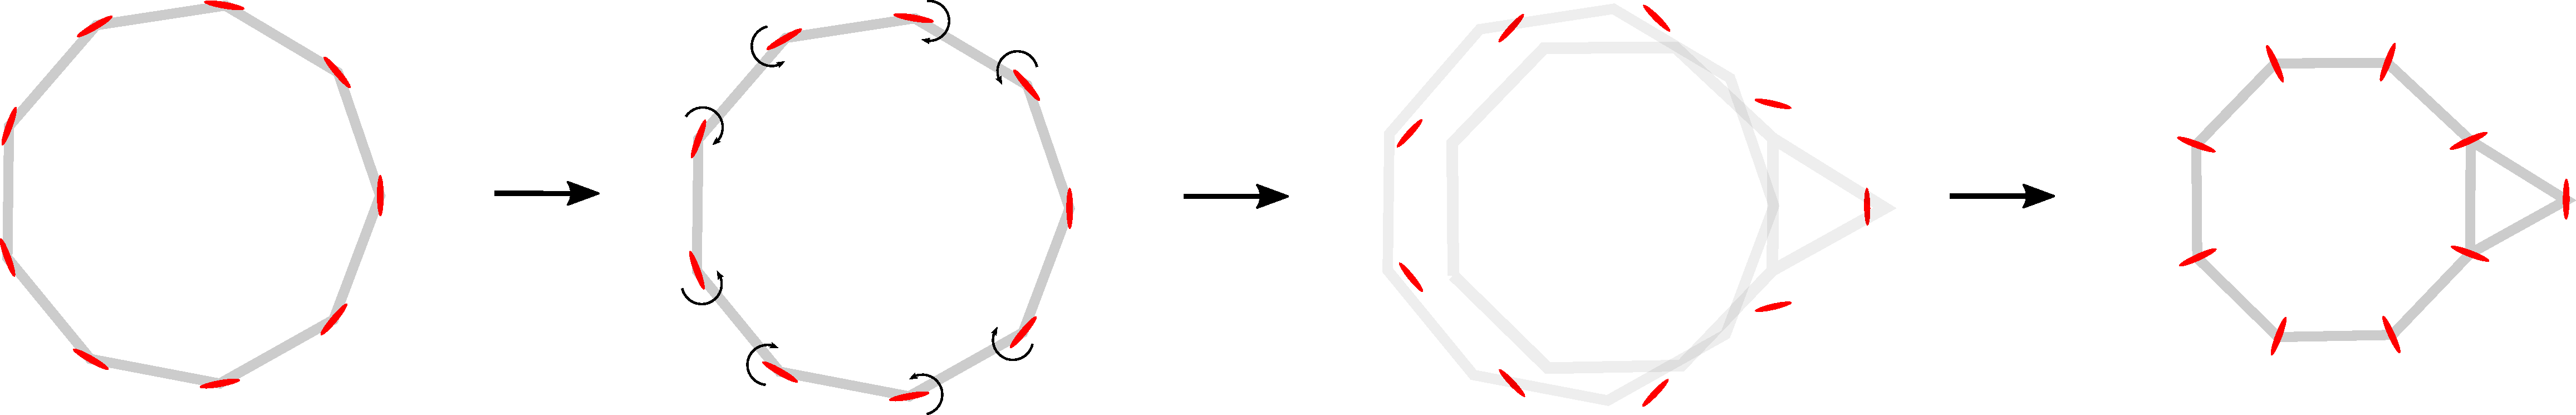
\includegraphics[width=12cm]{figures/3-elastic-figs/barriersScheme.pdf}
\caption{"Pop out" transition between two configurations.}
\label{fig:popout}
\end{figure}

\todo{What about the transition to the 5+3 configuration (i.e the pentagon+triangle), is the method + the barrier similar?}
\todo{Double check Jon's rope pulling?/at some point 'release' it akin to the peel}
\todo{what about the transition for fewer than 6 inclusions/more the 6 inclusions. Try a saimilar method and see what happend}
\todo{Verfiy with simple Monte Carlo stuff.}

\todo{Pull only in xy space and allow both xy angles and actually angles to vary.}

\todo{How does separation scale with tension? could that be a control parameter?}
}
\section{Multi-scale Model for Configurations}
So far, we have only considered the dynamics of inclusions that are initialised sufficiently far apart, such that the equilibrium configurations explore the stable equilibrium around \todo{R (get the right R)}. Inclusions that are separated by a distance less that \todo{this R} will be attracted together by the diverging interaction potential. As the inclusions come close together the separation $R/\epsilon\sim\mathcal{O}(1)$ and so we expect additional terms to appear in the expansion of the interaction potential\todo{if we still use the weak weak form, it just rescales the tension and thus the ratio e/R is still very small - needed for the weak-weak case. Should probably reword this.}. Physically, the inclusions cannot overlap and so we introduce a repulsive term that dominates at small $R$. Inspired by the form of the weak-weak interaction potential we add a term  that goes like $\epsilon^2\frac{4}{R^4}((\alpha_{1}^{(0)})^2+(\alpha_{2}^{(0)})^2)$ and using $\bar{E}=E\mu^2/\pi\alpha^2$ gives
\begin{equation}
\begin{split}
    \bar{E}_2(\bar{R}, \psi_1, \psi_2) &= 2K_0(\bar{R}) + 2\omega K_2(\bar{R})(\cos2\psi_1+\cos2\psi_2) \\
    &+\omega^2\cos(2(\psi_1-\psi_2))K_0(\bar{R})+\omega^2\cos(2(\psi_1+\psi_2))\left(K_4(\bar{R})-\frac{48}{\bar{R}^4}\right) + \epsilon^2\frac{8}{\bar{R}^4}
\end{split}
\end{equation}
This potential now diverges to positive infinity as $R \rightarrow 0$, and for small $\epsilon$, there exists a local minimum, $R_c$, at small separations. The minimum energy still corresponds to $\psi_1 = \psi_2 = \pi/2$ and the separation distance $R_c$ is a functions of $\epsilon$, $R_c=R_c(\epsilon)$. About this equibrlium, the potential is much is much steeper nearby, it is a stiffer equilibrium. Due to the gradients in energy around this minimum, the system's relaxation to equilibrium is therefore dominated by the energy landscape at small separations and intially we will see the dynamics of two inclusions that are in the collapsing regime rapidly converge to the close equilibrium separation, which we will call a \textit{close pair}. Each inclusion in the close pair of inclusions will feel the same forces from external inclusions to leading order in $R_c$ and so we expect the close pair to move together in response to external inclusion arrangments.

\subsection{Effective Super Pairs}
\todo{need to sort out all the $\phi$s vs $\psi$s, need to be consistent.}
The two inclusions close together will exert a strong force on each other and will have some new equilbrium orientation/separation. The new minimum is a much deeper well in the interaction energy, where the two inlcusions are aligned perpendicular to the line between them, but at a much closer separation $R^*_{C}$. Since this well is much deeper and \todo{narrower} than the further out equilibrium, the two inclusions in the close pair will feel strong restoring forces keeping them at this separation. 

We can describe the close pairs by the $x$, $y$ and $\phi$ coordinates describing each inclusion, however similar to interacting particles in an external field, we can also describe the inclusions in a centre of mass coordinate system. In this analogy, the external field is provided by the other far away inclusions which will exert a much smaller force on each inclusion in the pair compared to the force they experience from each other. A natural choice to parameterise the positional coordinates is therefore
\begin{equation}
\begin{split}
x_c = \frac{x_1+x_2}{2}, \quad\text{ and }&\quad y_c = \frac{y_1+y_2}{2} \\
r =  \sqrt{(x_1-x_2)^2+(y_1-y_2)^2}, \quad\text{ and }&\quad \theta = \tan ^{-1}(y_1-y_2,x_1-x_2).
\end{split}
\end{equation}
where describing the orientation of the super pairs is useful as this will be coupled to the individual inclusion alignment. A convenient treatment of the orientations will be to consider the average and difference between the orientations of the two separate inclusions. Simply taking the mean value of $\phi_1$ and $\phi_2$ does not calculate the average orientation in general. Consider two inclusions with $\phi_1=\pi/2-0.01$ and $\phi_2=-\pi/2+0.01$, where the angles describe two similarly orientated inclusions, $\updownarrow$ and $\updownarrow$. The arithmetic mean of this is gives $\phi_C=0$, which gives a very different orientation to both individual inclusions, $\leftrightarrow$ (this cannot be fixed by simply measuring the angles on the domain $0$ to $\pi$, as this simply rotates the problem case, $\phi_1=\pi-0.01$ and $\phi_2=0.01$). The solution is to measure the both angles within the same quadrant, as then the maximum angular difference between the two orientations will be $\pi/2$. Using the properties of the two argument $\arctan$, this can be written in general as
\begin{equation}
\begin{split}
\phi_c &= \frac{1}{2}\arctan\left(\cos2\phi_1+\cos2\phi_2,\sin2\phi_1+\sin2\phi_2\right) \quad\text{ and } \\
\phi_d &= \phi_1 - \phi_2
\end{split}
\end{equation}
where we allow $\phi_d$ to depend on how the separate angles were measured. \todo{discuss that the arctan thing is not actually going to be an issue...}

The new set of coordinates highlights the slow and enslaved variables. From the steep potential around the close equilibrium separation we expect that to leading order $r=R^*_c$ and $\phi_d=0$. We also expect that $\theta= \pi/2 + \phi_c$ and as such the pair of inclusions can be described by three slow variables. However it is not clear whether the gradients in $\phi_c$ or $\theta$ dominate the dynamics - whether the rotation of the pair is limited by the translational motion of the inclusions, or the rotation. Thus, simply setting $\theta= \pi/2 + \phi_c$ or $\phi_c = \theta - \pi/2$ may not capture the behaviour of the inclusion pair. To include both the translation and rotation of the individual inclusions when considering the motion of the pair, we take a linear combination of the two to eliminate the slow variable and define
\begin{equation}
    \psi_c = \frac{\theta + \kappa (\frac{\pi}{2} + \phi_c)}{1+\kappa} \quad\text{ and }\quad \psi_d = \theta - \left(\frac{\pi}{2} + \phi_c \right)
\end{equation}
where $\kappa$ is to be determined, $\psi_c$ gives the overall orientation of the pair and $\psi_d$ is enslaved by the fast variables to be zero.

The overdamped dynamics can be written as
\begin{equation}
    \frac{\dd \mathbf{X}_i}{\dd t}= \sum_{j}M_{ij}\frac{\dd E}{\dd \mathbf{X}_j},
\end{equation}
where we define the coordinate vector $\mathbf{X}=(x_1, x_2, y_1, y_2, \phi_1, \phi_2)$ and the mobility matrix, $\mathbf{M}=\mathrm{diag}(\mu_t, \mu_t, \mu_t, \mu_t,\mu_r, \mu_r)$. As a matrix equation this is
\begin{equation}
    \frac{\dd \mathbf{X}}{\dd t}= \mathbf{M}\frac{\dd E}{\dd \mathbf{X}}.
\end{equation}
Defining the new coordinate vector, $\mathbf{Y}=(x_c, y_d, \psi_c, r, \psi_d, \phi_d)$ and the Jacobian between these two coordinate systems, $\mathbf{J}$, the new variables will evolve in a similar fashion
\begin{equation}
    \frac{\dd \mathbf{Y}}{\dd t} = \mathbf{J}\frac{\dd \mathbf{X}}{\dd t} = \mathbf{J}\mathbf{M}\frac{\dd E}{\dd \mathbf{X}} = \underbrace{\mathbf{J}\mathbf{M}\mathbf{J}^{-1}}_{\mathbf{M'}}\frac{\dd E}{\dd \mathbf{Y}}.
\end{equation}
This gives the same evolution equation, but with a modified mobility matrix. Evaluating this new mobility matrix gives
\begin{equation}
    \mathbf{M}'=
\left(
\begin{array}{cccccc}
 \frac{\mu_t}{2} & 0 & 0 & 0 & 0 & 0 \\
 0 & \frac{\mu_t}{2} & 0 & 0 & 0 & 0 \\
 0 & 0 & \frac{\kappa ^2 \mu_r+\frac{4 \mu_t}{(x_{1}-x_{2})^2+(y_{1}-y_{2})^2}}{2 (\kappa +1)^2} & 0 & \frac{\frac{4 \mu_t}{(x_{1}-x_{2})^2+(y_{1}-y_{2})^2}-\kappa  \mu_r}{2 (\kappa +1)} & 0 \\
 0 & 0 & 0 & 2 \mu_t & 0 & 0 \\
 0 & 0 & \frac{\frac{4 \mu_t}{(x_{1}-x_{2})^2+(y_{1}-y_{2})^2}-\kappa  \mu_r}{2 (\kappa +1)} & 0 & \frac{\mu_r}{2}+\frac{2 \mu_t}{(x_{1}-x_{2})^2+(y_{1}-y_{2})^2} & 0 \\
 0 & 0 & 0 & 0 & 0 & 2 \mu_r \\
\end{array}
\right).
\end{equation}
Coupling $\theta$ and $\phi_c$ introduces off diagonal terms in the mobility matrix, that depend on the other coordinates in the system. However choosing $\kappa = 4\mu_t/(r^2\mu_r)$ these off-diagonal terms vanish and at the pair equilibrium we expect, $r=R_C^*$ which is constant and therefore we take $\kappa = 4\mu_t/((R_C^*)^2\mu_r)$.\todo{$\mu_r$ is larger, but $r$ is small, is this going to cause issues about the separation of the time scales?} \todo{Say about: $\kappa$ implies the relative contribution of each process in limiting the rotation of the pair} The mobility matrix is fully diagonal,
\begin{equation}
    \mathbf{M}'=\mathrm{diag}\left(\frac{\mu_t}{2},\frac{\mu_t}{2},\frac{2 \mu_r \mu_t}{r^2\mu_r+4\mu_t},2\mu_t,\frac{\mu_r}{2}+\frac{2 \mu_t}{r^2},2\mu_r\right)
\end{equation}
and we therefore have a reduced system where we set $r=R^*_C$, $\psi_d=0$, and $\phi_d=0$. We can evolve the remaining three variables, the \textit{reduced system}, describing the pair of inclusions using the overdamped dynamics, but with transformed mobilities.

In addition to the modified mobility, we need to calculate gradients of the energy in the reduced system. Using the general two body interaction energy $E_2(R, \psi_a, \psi_b)$ from \todo{equation} we label a configuration of $n$ inclusions with the inclusions $1$ and $2$ being in a close pair. The energy of the configuration with the pair is therefore
\begin{equation}
\begin{split}
    E_{overall} &= \left(\sum_{i=3}^{n}\sum_{i=j+1}^{n}E_{2}\big(R_{ij}, \psi_i-\theta_{ij}, \psi_j-\theta_{ij}\big)\right) + E_{2}\big(R_{12}, \psi_1-\theta_{12}, \psi_2-\theta_{12}\big)\\
    &+ \sum_{i=3}^{n}\Big(E_{2}\big(R_{i1}, \psi_i-\theta_{i1}, \psi_1-\theta_{i1}\big) + E_{2}\big(R_{i2}, \psi_i-\theta_{i2}, \psi_2-\theta_{i2}\big)\Big)
\end{split}
\end{equation}
where we split the interaction energy into contributions from inclusions not in the pair, inclusions in the pair, and an inclusion in the pair and interacting with an inclusions away from the pair. The first term is unaffected by the coordinate transformation. The second term is the interaction between the two inclusions in the pair and this term drives the fast dynamics in the system, constraining the pair of inclusions to be at their equilibrium separation and orientation. This contribution can be written as $E_{2}\big(R_{12}, \psi_1-\theta_{12}, \psi_2-\theta_{12}\big) = E_{2}\big(r, \pi/2, \pi/2\big)$ which will be constant for the slow dynamics. Since the inclusion in the pair are close together, that is $r \ll 1$, they are also close to $x_c$ and $y_c$ and so we can expand the energy around these points. For inclusion $1$ this is
\begin{equation}
\begin{split}
    E_{2}\big(R_{i1}, &\psi_i-\theta_{i1}, \psi_1-\theta_{i1}\big) = \\
    &E_{2}\big(R_{ic}, \psi_i-\theta_{ic}, \psi_c-\theta_{ic}\big) + \left[\left(\frac{\partial E_{2}}{\partial R}\frac{\partial R_{i1}}{\partial x_1}-\left(\frac{\partial E_{2}}{\partial \psi_a} + \frac{\partial E_{2}}{\partial \psi_b}\right)\frac{\partial \theta_{i1}}{\partial x_1}\right)\frac{r}{2}\cos\psi_{c}\right. \\
     &+ \left.\left(\frac{\partial E_{2}}{\partial R}\frac{\partial R_{i1}}{\partial y_1}-\left(\frac{\partial E_{2}}{\partial \psi_a} + \frac{\partial E_{2}}{\partial \psi_b}\right)\frac{\partial \theta_{i1}}{\partial y_1}\right)\frac{r}{2}\sin\psi_{c}\right]_{R=R_{ic}, \psi_a=\psi_i-\theta_{ic}, \psi_b=\psi_c-\theta_{ic}} + \mathcal{O}(r^2)
\end{split}
\end{equation}
where we have $R_{ij} = \sqrt{(x_i-x_j)^2+(y_i-y_j)^2}$ and $\theta_{ij}=\arctan(x_i-x_j, y_i-y_j)$. We can do the same thing for inclusion $2$ which gives an identical expansion except with $r\rightarrow-r$ and so the linear terms in the expansion exactly cancel out in the expansion \todo{Can we write this r/R ? I dont think that is what is it actually...}. As such we can now write the energy as
\begin{equation}
\begin{split}
    E_{overall} &= \left(\sum_{i=3}^{n}\sum_{i=j+1}^{n}E_{2}\big(R_{ij}, \psi_i-\theta_{ij}, \psi_j-\theta_{ij}\big)\right) + \sum_{i=3}^{n}2E_{2}\big(R_{ic}, \psi_i-\theta_{ic}, \psi_c-\theta_{ic}\big) + \mathcal{O}(r^2)
\end{split}
\end{equation}
where the energy has been shifted by the self interaction energy of the inclusion pair. In fact this procedure can be generalised so that the interaction of multiple pairs of inclusions can also be described, where two interacting pairs of inclusions contribute $4 E_{2}\big(R_{ic}, \psi_i-\theta_{ic}, \psi_c-\theta_{ic}\big)$ to the total interaction energy. Recall that we scaled the interaction energy by the magnitude of the monopole mode. An inclusion with the same asymmetry, but different couple the induced curvature would contribution twice as much to the interaction energy which is exactly the effect of the inclusion pair, upto $\mathcal{O}(r^2)$. We can therefore model a pair of inclusions as one single inclusion, with the same anisotropy but twice the monopole mode and a modified translational and rotational mobility \todo{check that we've used $\theta_c$ or $\psi_c$ or whatever at the right time}.

\todo{we expect that increaseing e.g. the mean curvature would icncrease the footprint anad affect the mobility?}

The reduced system can be used to evolve a random configuration of inclusions, that also includes pairs of inclusions that are close together. The pair-to-inclusion and pair-to-pair interactions have the same features as the inclusion-to-inclusion interaction and so we expect that resulting stable configurations will also have similar structure. This is in fact what we find. Resulting stable configurations of inclusions and pairs, have the same polygonal structure, with slight perturbations due to the increased strength of the pair interactions. However, depending an the initial configuration a system containing a par of inclusions might converge to a different final configuration when compared to single inclusions that are initialised with the same starting configuration.
m
\todo{We could do a similar analysis for groups of e.g. three inclusions, but we are focusing on the well separated limit which its unlikely that multiple inclusions will be stuck together.}

\notyet{
\subsection{Effective Super Pairs}  

Could be useful for polymerising systems? \cite{saletti_matrix_2017}

The dynamics of two interacting particles in an external potential can be described as
\begin{align}
    m_1\ddot{\mathbf{r}}\mathbf{_1} = \textbf{F} + \nabla_{\mathbf{r}\mathbf{_1}}E_{\text{ext}} \\
    m_2\ddot{\mathbf{r}}\mathbf{_2} = -\textbf{F} + \nabla_{\mathbf{r}\mathbf{_2}}E_{\text{ext}}
\end{align}
where we can assume the interaction giving the force $\textbf{F}$ is conservative to give so we can define an additional term in the external energy that depends on $(\mathbf{r}\mathbf{_1}-\mathbf{r}\mathbf{_2})$ and consequently the gradient in the different variables picks up the change of sign.
\begin{align}
    m_1\ddot{\mathbf{r}}\mathbf{_1} = \nabla_{\mathbf{r}\mathbf{_1}}E \\
    m_2\ddot{\mathbf{r}}\mathbf{_2} = \nabla_{\mathbf{r}\mathbf{_2}}E
\end{align}
 where $\textbf{F}$ is the equal an opposite force extered by one particle on the other and $E$ is the external potential. Making the transformation in a 1d system, to centre of mass and \textit{difference} coordinates, we write
 \begin{equation}
 \underbrace{\left(
\begin{array}{cc}
 x_C \\
 x_d \\
\end{array}
\right)}_{\textbf{y}} = \underbrace{\left(
\begin{array}{cc}
 \frac{m_1}{m_1+m_2} & \frac{m_2}{m_1+m_2} \\
 1 & -1 \\
\end{array} \right)}_{M} \cdot \underbrace{\left(
\begin{array}{cc}
 x_1 \\
 x_2 \\
\end{array} \right)}_{\textbf{x}}.
\end{equation}
so $y_i = \sum_j M_{ij}x_j$ and thus $\partial y_i / \partial x_j = M_{ij}$ Defining $L=\text{diag}(m_1, m_2)$ we can rewrite the dynamics
\begin{equation}
    \ddot{y}=M \ddot{x}=M L^{-1}\nabla_{\mathbf{x}}E.
\end{equation}
Using the transform 
\begin{equation}
    (\nabla_x E)_i = \frac{\partial E}{\partial x_i} = \sum_j \frac{\partial E}{\partial y_j}\frac{\partial y_j}{\partial x_i} = \sum_j \frac{\partial E}{\partial y_j} M_{ji} = (M^T \nabla_y E)_i
\end{equation}
so $\ddot{y}= M L^{-1} M^T\nabla_{\mathbf{y}}E$ and we therefore define a new effective mass matrix $L_y = (M L^{-1} M^T)^{-1}$ which for the $L$ and $M$ defined above we find
\begin{equation}
    L_y = \left(
\begin{array}{cc}
 m_1+m_2 & 0 \\
 0 & \frac{m_1 m_2}{m_1+m_2} \\
\end{array}
\right)
\end{equation}
which is the usual total and reduced mass. For the overdamped evolution, we consider $\dot{x}=\mu_x\nabla_x$ and for a transformed variable $y$, we get $\mu_y = M\mu_xM^T$. Using the uniform expansions, we expect two inclusions that have been brought together will form a stiff inclusion pair separated by a much smaller equilibrium distance, $r_C$. We can define new transformed variables that describe the position of the centre of mass and relative distance of both spatial coordinate in the system, as well as the angular coordinates. (I think that these coordinated fundamentally miss the coupling between the position and angle.) So we have $v_c = (v_1 + v_2)/2$ and $v_d = (v_1 - v_2)$. The transformation matrix for all three coordinates looks like    
\begin{equation}
    M = \left(
\begin{array}{cccccc}
 \frac{1}{2} & \frac{1}{2} & 0 & 0 & 0 & 0 \\
 1 & -1 & 0 & 0 & 0 & 0 \\
 0 & 0 & \frac{1}{2} & \frac{1}{2} & 0 & 0 \\
 0 & 0 & 1 & -1 & 0 & 0 \\
 0 & 0 & 0 & 0 & \frac{1}{2} & \frac{1}{2} \\
 0 & 0 & 0 & 0 & 1 & -1 \\
\end{array}
\right)
\end{equation}
and we have
\begin{equation}
    \mu_x = \left(
\begin{array}{cccccc}
 \mu_t & 0 & 0 & 0 & 0 & 0 \\
 0 & \mu_t & 0 & 0 & 0 & 0 \\
 0 & 0 & \mu_t & 0 & 0 & 0 \\
 0 & 0 & 0 & \mu_t & 0 & 0 \\
 0 & 0 & 0 & 0 & \mu_r & 0 \\
 0 & 0 & 0 & 0 & 0 & \mu_r \\
\end{array} \right)
\quad
\text{and}
\quad
 \mu_y = \left(
\begin{array}{cccccc}
 \frac{\mu_t}{2} & 0 & 0 & 0 & 0 & 0 \\
 0 & 2 \mu_t & 0 & 0 & 0 & 0 \\
 0 & 0 & \frac{\mu_t}{2} & 0 & 0 & 0 \\
 0 & 0 & 0 & 2 \mu_t & 0 & 0 \\
 0 & 0 & 0 & 0 & \frac{\mu_r}{2} & 0 \\
 0 & 0 & 0 & 0 & 0 & 2 \mu_r \\
\end{array}
\right)
\end{equation}

Consider a system of two close inclusions and one far away. We write the energy in a similar form the two body problem, for $E = E_{12}+E_O$, where $E_{12}$ describes the interaction energy between the two close inclusions and $E_O = E_{13}+E_{23}$. Consider for example the evolution of $x_C = (x_1 + x_2)/2$.  We know
\begin{equation}
    \frac{\partial E_{12}}{\partial x_{1}} = -\frac{\partial E_{12}}{\partial x_{2}}
\end{equation}

...

A better set of transforms will be to use the following


\begin{center}
$\begin{array}{ |c|c| }
\hline
\textbf{New Vars} & \textbf{Old Vars} \\
\hline
x_c & \frac{x_1+x_2}{2} \\
y_c & \frac{y_1+y_2}{2} \\
r & \sqrt{(x_1-x_2)^2+(y_1-y_2)^2} \\
\theta & \tan ^{-1}(y_1-y_2,x_1-x_2) \\
\phi_c & \frac{\phi_1+\phi_2}{2} \\
\phi_d & \phi_1-\phi_2 \\
\hline
\end{array}$
\end{center}
however these are not linear and so to the transformation will not be a constant matrix. We make a transform using the Jacobian

$\left(
\begin{array}{cccccc}
 \frac{1}{2} & \frac{1}{2} & 0 & 0 & 0 & 0 \\
 0 & 0 & \frac{1}{2} & \frac{1}{2} & 0 & 0 \\
 \frac{x_1-x_2}{\sqrt{(x_1-x_2)^2+(y_1-y_2)^2}} & -\frac{x_1-x_2}{\sqrt{(x_1-x_2)^2+(y_1-y_2)^2}} & \frac{y_1-y_2}{\sqrt{(x_1-x_2)^2+(y_1-y_2)^2}} & -\frac{y_1-y_2}{\sqrt{(x_1-x_2)^2+(y_1-y_2)^2}} & 0 & 0 \\
 \frac{y_1-y_2}{(x_1-x_2)^2+(y_1-y_2)^2} & -\frac{y_1-y_2}{(x_1-x_2)^2+(y_1-y_2)^2} & \frac{x_2-x_1}{(x_1-x_2)^2+(y_1-y_2)^2} & -\frac{x_2-x_1}{(x_1-x_2)^2+(y_1-y_2)^2} & 0 & 0 \\
 0 & 0 & 0 & 0 & \frac{1}{2} & \frac{1}{2} \\
 0 & 0 & 0 & 0 & 1 & -1 \\
\end{array}
\right)$
which result in the modified mobilities
\begin{equation}
    \left(
\begin{array}{cccccc}
 \frac{\mu_t}{2} & 0 & 0 & 0 & 0 & 0 \\
 0 & \frac{\mu_t}{2} & 0 & 0 & 0 & 0 \\
 0 & 0 & 2 \mu_t & 0 & 0 & 0 \\
 0 & 0 & 0 & \frac{2 \mu_t}{r^2} & 0 & 0 \\
 0 & 0 & 0 & 0 & \frac{\mu_r}{2} & 0 \\
 0 & 0 & 0 & 0 & 0 & 2 \mu_r \\
\end{array}
\right)
\end{equation}
The new set of coordinates highlights the slow and enslaved variables. From the steep potential around the close equilibrium separation we expect that to leading order $r=R^*_c$ and $\phi_C$. We also expect that $\phi_d = \pi - \theta$. Without looking at the energy gradients, it's not obvious whether the gradients in $\phi_d$ or $\theta$ dominate the dynamics. As such we can take a linear combination of the two to define two new variables
\begin{center}
$\begin{array}{ |c|c| }
\hline
\textbf{New New  Vars} & \textbf{New Vars} \\
\hline
\theta_b & (\theta + \kappa (\pi - \phi_c))/(1+\kappa) \\
\phi_0 & \theta - (\pi - \phi_c) \\
\hline
\end{array}$
\end{center}
where we choose $\kappa$ such that the mobilities are kept to be diagonal. This occurs when $\kappa = 4\mu_t/(r^2\mu_r)$, which slightly complicates the mapping since $\kappa$ depends on one of the new variables. Instead, we use the equilibrium value of $r=R^*_C$ to make the transformed mobility diagonal when the $r$ variable equilibrates, which we expect to happen very quickly due to the steep potential. We therefore have a reduced system where we set $r=R^*_C$, $\phi_0$, and $\phi_d=0$. We can evolve the remaining three variables, the \textit{reduced system}, describing the pair of inclusions using the overdamped dynamics, but with transformed mobilities. If the inclusions in the pair were not at the equilibrium separation, there would be a small error in the dynamics, but comparing the solutions to both the full system and the reduced system showed very good agreement.
}

\section{Discussion and Conclusions}

This work has focused on a specific limit of the membrane mediated interaction between curvature inducing inclusions: when the inclusions induce small curvatures and when the inclusions are far apart. This is a previously understudied regime, with many models considering inclusions that are much closer together. In the well separated limit considered here the effects of the membrane elasticity dominate, without near field interactions, such as steric effects, or changes to the bilayer thickness from the protein binding (we expect this variation to decay exponentially) \todo{cite}.

The anisotropy in the system fundamentally changes the interaction by the introduction of an equilibrium separation, rather than infinite repulsion for the symmetric case. Furthermore, the anisotropy has an effect in the formation of aggregates of inclusions. Typically, an interaction with an equilibrium separation, but no orientation dependence will form a triangular packing \todo{cite, could simulate with $\omega=0$} however this can induce geometric frustrations if the interaction depends on the particles are aligned, which is again due to the anisotropy. In fact, the formation of the polygonal lattices observed here could be general to any potential with a monopole-quadrupole or quadrupole-quadrupole interaction.

Mean field descriptions of systems comprised of anisotropic particles have been developed in the past. Such theories aim to describe the key features of inter-inclusion interaction as a function of some order parameter that depends on average behaviour within a region. A pertinent and simple example is the Maier–Saupe theory of liquid crystals. The theory defines a director that captures the average orientation of a small coarse-grained region and introduces an energetic cost to gradients in this director, assuming some potential that acts to align the director field. As such, a distribution of particles can be modelled by the director field without tracking each individual particle. However in the lattices studied here, we find that in the aggregates of inclusions, the alignment of inclusions vary between neighbouring inclusions and this variation is not regular. Models of a director field would therefore need to keep track of every inclusion and this would limit the ability of the model to describe a larger number of inclusions. In the ring configurations that comprise the lattice, inclusions are placed at equally spaced angles. We therefore expect the distribution of angles from a very large lattice to be uniform over angle and as such, the average induced curvature of the aggregate will be the monopole mode. At this scale, the continuum models of isotropic curvature may still provide a useful description for a much broader class of inclusions (even those with anisotropy).
\notyet{


\begin{itemize}
    \item this is a fundamentally discrete model - connect to continuum models perhaps?
    \item what could the interaction mean for e.g. engineering?
    \item when is this going to be relevant for bio? is it? synthetic bio?
\end{itemize}


Aggregation of BAR proteins has been observed in many contexts, with characteristic features that can depend on physical properties on the system, for example the protein density or the membrane tension. In this work, we assume that the inter-inclusion separation is much larger than the inlcusion size and so the volume fraction of the system is very low. This \todo{prevents this mechanism and this mechanism as observed here}. However, the \todo{cite} identifies that the lattice structure formed at low protein volume fractions is affected by the membrane tension. Here, we define the dimnesionless parameter $\mu=\sqrt{\kappa/TL^2}$ where $L^2$ is the average inclusions separation. As the average separation between inclusions increases this is equivalent to decreasing the membrane tension.

\section{Sensing and Scaffolding}

At low densities, BAR domain proteins have been identified as sensing membrane curvature and responding 

What would the parameters actually be for a BAR protein?
How does this affect?
Numbers on volume fractions? (and therefore errors?)

"BAR-membrane interactions depend not only on the structures of the proteins, but also on membrane shape and tension, as well as protein densities on the membranes" \cite{tsai_comparing_2021}

Aggregation of BAR proteins has been observed in many contexts, with characteristic features that can depend on physical properties on the system, for example the protein density or the membrane tension. In this work, we assume that the inter-inclusion separation is much larger than the inlcusion size and so the volume fraction of the system is very low. This \todo{prevents this mechanism and this mechanism as observed here}. However, the \todo{cite} identifies that the lattice structure formed at low protein volume fractions is affected by the membrane tension. Here, we define the dimnesionless parameter $\mu=\sqrt{\kappa/TL^2}$ where $L^2$ is the average inclusions separation. As the average separation between inclusions increases this is equivalent to decreasing the membrane tension.

(this is still much higher no? so need to talk about the general principle, not specific ones I think).

Lots of this from thinking about \cite{simunovic_when_2015}.

\section{Membrane Tubules and Future Work}

Elastic interactions between curvature inducing membrane bound inclusions can create interesting many body dynamics. The interactions and dynamics explored so far in this transfer thesis were all based on three assumptions of the system: the membrane has no intrinsic curvature, the tension and anisotropy are $\mathcal{O}(1)$ and the inclusions are far apart. However the BAR domain family of proteins has been linked to the process of membrane tubule formation and can form scaffolds on the cylindrical surface of the tubule.\cite{le_roux_dynamic_2021}

Theories describing the formation of these membrane tubule scaffolds are starting to explore the role of the anisotropy in many membrane bound proteins.\cite{noguchi_binding_2022} Noguchi, Tozzi and Arroyo showed that as protein density increase, the alignment of proteins exhibit a transition to an ordered state on both flat and tube-like membranes.\cite{noguchi_binding_2022} Volume exclusion is a driving force in this transition from a disordered to nematic state and the anisotropy of the protein causes a preferred alignment on cylindrical structures to match the curvature and minimise the bending energy. The elastic effects however were not considered in detail. The elastic energy used assumes a fixed cylindrical geometry such that the surface is entirely described by a radius $R_{cy}$ (and therefore principle curvatures $1/R_{cy}$ and $0$) and length $L_{cy}$. However, finite sized inclusions embedded in the membrane will likely form perturbations to this specific shape and the membrane could mediate an interaction similarly to those studied on the flat plane. Using the same system setup as described earlier in this chapter, a similar procedure of deriving a shape equation and solving for the resulting shape would give the interaction energy of the system. Since the membrane is no longer rotationally invariant, the interaction is expected depend additionally on the axis of the cylinder.

Challenges in directly imaging BAR domain proteins have prevented the lack of detailed understanding of tubule formation mechanisms, however the structure of helical scaffolds wrapping around these tubules have been resolved.\cite{mim_structural_2012, frost_structural_2008} These structures show that the formation of helices on membrane tubules are influenced by chemical tip-to-tip interactions between the elliptical bar proteins. This scaffold presents a much denser limit, where inclusions are much more closely packed, hence motivating the use of volume exclusion effects\cite{noguchi_binding_2022}. This limit is a very different regime to study the elastic interactions compared to the large separation limit. However understanding how the closeness of the inclusions and the how tightly coiled the helix is would provide insight into how membrane tubules and the subsequent protein scaffolds would form.

\section{Needs to go somewhere}

\subsubsection{Biophysical Parameter Values}

The bending stiffness, $\kappa$, of lipid bilayer membranes are typically of around $30 k_B T \approx 1 \times 10^{-19} $ J \cite{weikl_interaction_1998} and can have a range of tensions, typically from $0.003$-$0.3\text{mNm}^{-1}$. \cite{shi_membrane_2015} If we set $\mu=1$ we find that $L = \sqrt{\kappa/T} \sim$ which gives the range of $L$ as $1.8\times10^{-8}$-$1.8\times10^{-7}m$. The radius of typical BAR domains is $5-10$nm, giving a range of $\epsilon = 0.56-0.028$. Using the structure of BAR domain proteins the contact angle $\alpha$ looks to be around $0.772-0.394$. Cells are typically of size $10^{-5}-10^{-4}$m.

This is when measured in the inner coordinate system (so dont need to do the transformation..?)

We write $E= TA_0 + \kappa\xi^2 E'$ with $E'$ as the interaction energ
\cite{weikl_interaction_1998}: $\kappa\approx1\times10^{-19} J$, $\alpha\approx0.5$ (26.8degrees), $a=4nm$ (radius of inclusion). Something about the convergence of of the interaction at the top of 57 and that small deformations is similar to  strong tension? need to think about this a bit I think, tension of $=1mN/m$ is below the known rupture limit

\cite{galatola_many-body_2023}: $a\approx5nm$, $\alpha=10$ to $35 degrees$, $\kappa$ typically $30 k_B T$

for $\mu$=1,  $L \sim \sqrt{\kappa/T} \sim \sqrt{10^{-19}/10^{-6}}=3.6\times10^{-7}m$

Cells can typically scale from $10$s to $100\mu m$.

Use Nocuggi and Fournier to find values of $\xi$ for our systems/the anisotropy?

\cite{shi_membrane_2015}: Interesting results on membrane tension coupling to instabilities - could tension rescale the curvavture? and thus no stable minimum? 
Tension quoted as between $0.003mNm^{-1}$ 1 to around $0.3mNm^{-1}$.

\subsubsection{Strange length scaling:}

Ultimately, the energy we find that the non-dimensionalised energy  $E'$ goes like $\sim \frac{\alpha_{i}^{l}\alpha_{i}^{k}}{\mu^2} \sim \alpha_{i}^{l}\alpha_{i}^{k}\frac{TL^2}{\kappa}$ and is connected to the energy of the full system via $E= TA_0 + \kappa\xi^2 E'$, so $\Delta E \sim \kappa \alpha_{i}^{l}\alpha_{i}^{k}\frac{\xi^2TL^2}{\kappa}$. Remembering that $\alpha_i$ is rescaled such that the height function is of $\mathcal{O}(1)$, we find that $\Delta E \sim \kappa\xi^2\frac{\epsilon^2}{\xi^2}\alpha_{i}^{l}\alpha_{i}^{k}\frac{TL^2}{\kappa} = TL^2\epsilon^2$
}
